\newcommand{\name}{A246 -- Laser Spectroscopy }
\documentclass[11pt,a4paper,notitlepage]{scrartcl}
\usepackage{DasPaket}
\title{ Advanced Laboratory Course}
\subtitle{\name  \\ \hrulefill}
\date{May 6th 2021 \\}
%\date{Date of Experiment \\ \sectionlinetwo{black}{88}}
\author[*]{\textsc{Dominic Schüchter}}
\author[$\dagger$]{\textsc{Jakob Krause}}
\affil[*]{\href{mailto:dschuechter@uni-bonn.de}{\faEnvelope  \hspace*{0.1cm}\texttt{dschuechter@uni-bonn.de}} {\color{black}$|$} \href{https://github.com/dschuechter}{\faGithub  \hspace*{0.1cm}\texttt{dschuechter}}}
\affil[$\dagger$]{\href{mailto:krause.jakob@uni-bonn.de}{\faEnvelope  \hspace*{0.1cm}\texttt{krause.jakob@uni-bonn.de}} {\color{black}$|$} \href{https://github.com/krausejm}{\faGithub  \hspace*{0.1cm}\texttt{krausejm}}}
\usepackage{blindtext}
\usepackage{cleveref}
\usepackage{booktabs}
\graphicspath{{figs/}}
\addbibresource{Literatur.bib}

\begin{document}

\maketitle
\vspace{-.8cm}
\thispagestyle{empty}
\begin{center}

\vspace{-.2cm}

\rule{12cm}{1pt} \\\vspace{-.6cm} \rule{10cm}{1pt}
\end{center}



\begin{abstract}
	In this report we investigate the $D_1$ transitions in natural Rb vapor cells. We build a linear absorption spectroscopy setup as well as non linear saturated absorption spectroscopy setup employing a diode laser. The hyperfine coupling constants of the Rb ground state and first excited state will be determined. Further on we verify the law of \textsc{Lambert-Beer} and give an estimate of the saturation power of $^{87}$Rb. We also study the dependence of laser output power on injection current.
\end{abstract}
\begin{center}
	 \rule{10cm}{1pt} \\\vspace{-.7cm} \rule{12cm}{1pt}
\end{center}

\setcounter{page}{-1}
\newpage

\tableofcontents
\thispagestyle{empty}
\newpage
\section{Introduction}
In this experiment we investigate the properties of a diode laser and will use it for high resolution laser spectroscopy setups. With these the hyperfine structure of Rb is studied. First we give the theoretical background necessary in section \ref{sec:theory}, after which we describe the experimental setup(s) in section \ref{sec:exp}. We show our measurements and analysis, consisting of examining diode laser characteristics, use of a \textsc{Fabry-Pèrot}-interferometer (FPI) as well as linear and non-linear absorption spectroscopy of the $D_1$ $(5S_{1/2}\to5{P_{1/2}})$ transition in Rb in section \ref{sec:anal}. Finally we draw conclusions in section \ref{sec:conc}.
\newpage
\section{Theory}
\label{sec:theory}
In the following we introduce shortly the theory of hyperfine-splitting in Atoms and the concepts of linear and non-linear absorption spectroscopy.
\subsection{Hyperfine structure of Rubidium}
Solving the (spinless) \textsc{Schrödinger} equation for an atom $$\hat{H}\psi(r,\theta,\varphi)=E\psi(r,\theta,\varphi),$$
where $\hat{H}$ contains only a kinetic term and the \textsc{Coloumb} potential results in three quantum numbers $$\hat{H}\ket{nlm}=E\ket{nlm}.$$
If we consider that electrons as well as nuclei carry spin, corrections can be calculated perturbatively. The interaction of the internal magnetic field with the spins of the electrons leads to corrections referred to as \emph{fine structure} while the interaction of nuclear spin with internal magnetic fields is called \emph{hyperfine structure}. The corrections to the original energy levels are given by \begin{equation}
	\label{eq:hfs}
	\Delta E_{\text{HFS}}=\frac{A_\text{HFS}}{2}\left[F(F+1)-J(J+1)-I(I+1)\right],
\end{equation}
where $I$ is the nuclear spin, $\mathbf{J}=\mathbf{L}+\mathbf{S}$ the total angular momentum of electrons and $\mathbf{F}=\mathbf{J}+\mathbf{I}$
is the total angular momentum of the atom. $A=A(nL_J)$ is the hyperfine structure constant \cite{demtröder,manual}. Figure \ref{fig:hfs} shows the ground state and first excited state of two different Rb isotopes including the hyperfine splitting which was discussed above.
\begin{figure}[htbp]
	\centering
	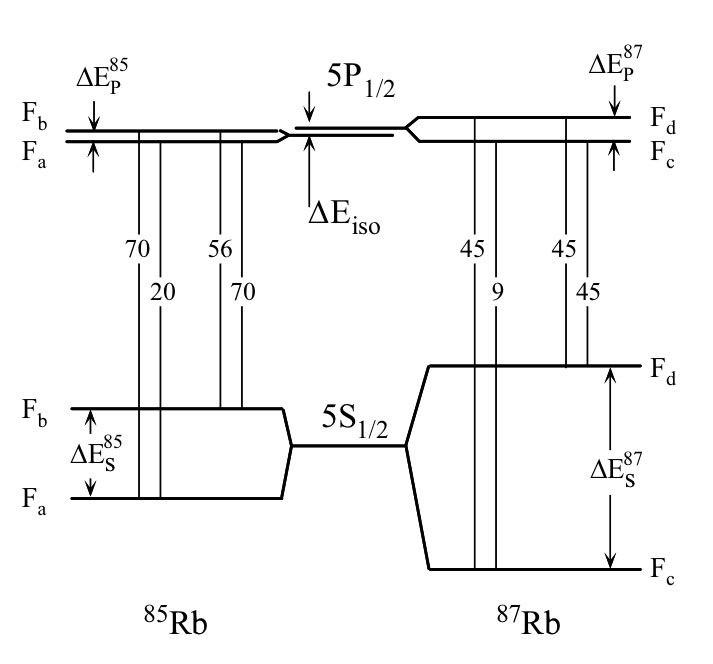
\includegraphics[width=.5\linewidth]{figs/experimental_setup/hfs.jpg}
	\caption{Possible hyperfine transitions in Rb with transition probabilities. Note that $F_a=2,F_b=3,F_c=1,F_d=2$. Taken from \cite{manual}}
	\label{fig:hfs}
\end{figure}
Because of different nuclear spin ($I(^{85}\text{Rb})=5/2$, $I(^{87}\text{Rb})=3/2$ \cite{85d,87d}) the hyperfine splitting is slightly different. Also the different \textsc{Coulomb} interactions in the isotopes account for the \emph{isotope shift} $\Delta E_\text{iso}$. The transition $5S_{1/2}\to5{P_{1/2}}$ ($D_1$ transition) will be studied with absorption spectroscopy setups using Rb vapor cells containing the natural mixture of $^{85}$Rb and $^{87}$Rb which is $\approx 3:1$ in favor of $^{85}Rb$ \cite{manual}. The wavelength belonging to the $D_1$ transition is around \SI{794}{\nano\m} \cite{manual}.

\subsection{Linear absorption spectroscopy}
If a plane wave transverses through a medium of two level atoms with length $L$ the transmission intensity decreases according to the \textsc{Lambert-Beer} law \cite{manual} \begin{equation}
	T(\nu)=e^{-\alpha(\nu)L},
	\label{eq:beer}
\end{equation}
where $\alpha(\nu)$ is the frequency dependent \emph{absorption coefficient}. For linear media ($\alpha L\ll 1$) the absorption coefficient can be written as \cite{manual} \begin{equation}
	\label{eq:lorentz}
\alpha(\nu)=\alpha_0\frac{(\Delta\nu/2)^2}{(\nu-\nu_0)^2+(\Delta\nu/2)^2},
\end{equation}
which is a \textsc{Lorentz} profile. Here $\Delta\nu$ is the \emph{natural linewidth}, which gives the lifetime $\tau$ of the excited state via \cite{manual} \begin{equation}
	\label{eq:lifetime}
	\tau=\frac{\hbar}{\Gamma}=\frac{1}{2\pi\Delta\nu}.
\end{equation}
However for $T>0$ there is atomic motion and common experimental absorption setups fail to measure the natural linewidth. Instead the \textsc{Doppler} broadened line profile is seen, which is described by the convolution of the \textsc{Lorentz}-profile with the \textsc{Maxwell} velocity distribution which results in a \textsc{Gaussian} \begin{equation}\label{eq:dopp}
	\alpha(\nu)=\alpha_0\exp\left[-\frac{(\nu-\nu_0)^2}{2\Delta\nu_D^2}\right],
\end{equation}
where $$\Delta\nu_D=\nu_0\sqrt{\frac{kT}{m_{\text{atom}}c^2}}$$ is the \textsc{Doppler} width \cite{manual}.
\subsection{Non-linear absorption spectroscopy}
In this experiment we make use of \emph{saturated} absorption spectroscopy as means of non-linear spectroscopy.
\subsubsection{Saturation of optical transitions}
Saturation refers to the event when a significant fraction of atoms in a two level medium is in the excited state. Thus modifying the absorption coefficient such that the medium seems more transparent since the absorption is proportional to the difference in population in excited and ground state \cite{manual}. Quantitatively one deals with this by defining the \emph{saturation parameter} $S$ which is defined as the fraction of power to saturation power \begin{equation}\label{eq:spar}
	S:=\frac{P}{P_{sat}}.
\end{equation}
The nonlinear absorption coefficient is then given by \begin{equation}\label{eq:nonlinear}
	\tilde{\alpha}(\nu)=\alpha_0\frac{(\Delta\nu/2)^2}{(\nu-\nu_0)^2+(\Delta\nu/2)^2(1+S)},
\end{equation}
which can be interpreted as power dependent \textsc{Lorentzian} with width \begin{equation}\label{eq:powernu}\Delta\nu(S)=\Delta\nu\sqrt{1+S}.\end{equation}
This is called \emph{optical power broadening}. \cite{manual}
The absorbed power in a \textsc{Doppler} broadened medium can be written as \cite{manual} \begin{equation}
		\Delta P\propto\frac{S}{\sqrt{1+S}}.
		\label{eq:power}
	\end{equation}
\subsubsection{Saturated absorption spectroscopy}
The experimental realization of saturation spectroscopy employs two counter propagating laser beams of the same frequency; a strong beam referred to as the pump beam which has at least the power $P>P_{sat}$ and a weaker probe beam. Figure \ref{fig:bennet} shows the effect of this experimental setup; the pump beam with frequency $\nu$ will excite a fraction of atoms which correspond to a "burnt hole" in the absorption profile. If the probe beam is not tuned to the same frequency as the pump beam it will not see the modified absorption. However on resonance, meaning that pump and probe frequency are the same, the two beams interact with the same class of atoms, namely those with zero velocity. This results in a modified absorption spectrum around the resonance frequency; a peak with the natural linewidth (called a \textsc{Lamb} dip). Thus, \textsc{Doppler} free spectroscopy is possible. \cite{manual}


\begin{figure}[htbp]
	\centering
	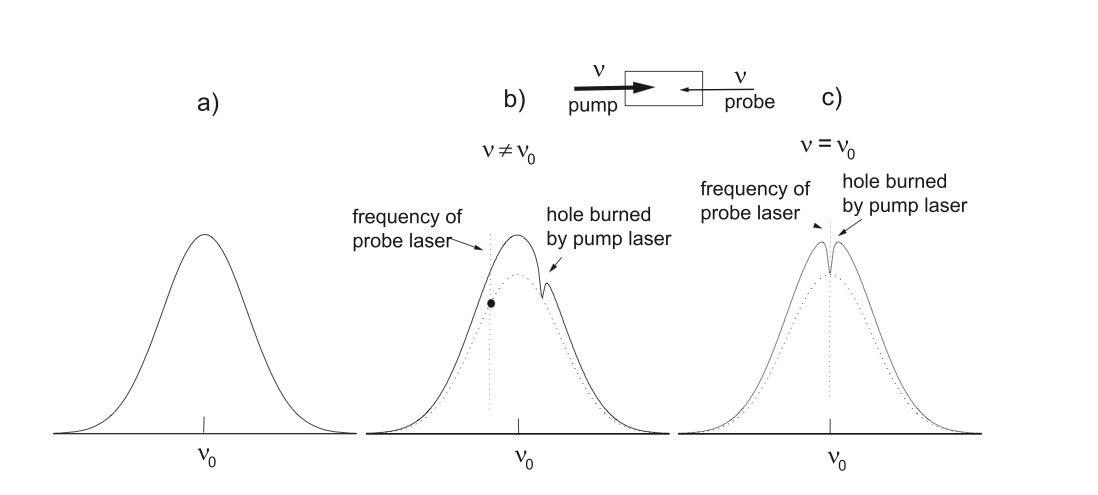
\includegraphics[width=.8\linewidth]{figs/experimental_setup/bennet.jpg}
	\caption{Consequences for the absorption profile if one employs probe beam and pump beam \cite{manual}}
	\label{fig:bennet}
\end{figure}

If we consider an optical transition where two excited states are possible separated less then a \textsc{Doppler} width these two transition can be made visible with saturated absorption spectroscopy. Naively one would expect two \textsc{Lamb} dips emerging from the \textsc{Doppler} broadened absorption profile; but not only two but actually three \textsc{Lamb} dips can be observed. The third dip observed lies exactly between the two individual lines and is called a "cross-over resonance". Atoms moving at a velocity such that the pump beam is at resonance with one transition and the probe beam with the other transition are the reason for the observation of crossover resonances. \cite{manual}


\section{Experimental Setup}
\label{sec:exp}
For the following measurements we had to build up different setups after one another. In this section we will explain the functionality of the used laser system and the \textsc{Fabry-Perot}-Interferometer (FPI). This section is based on the lab manual \cite{manual}. For more information on lasers or FPI's see \cite{laser} or \cite{}.
\subsection{L.A.S.E.R.}
\begin{wrapfigure}{R}{0.45\textwidth}
	\centering
	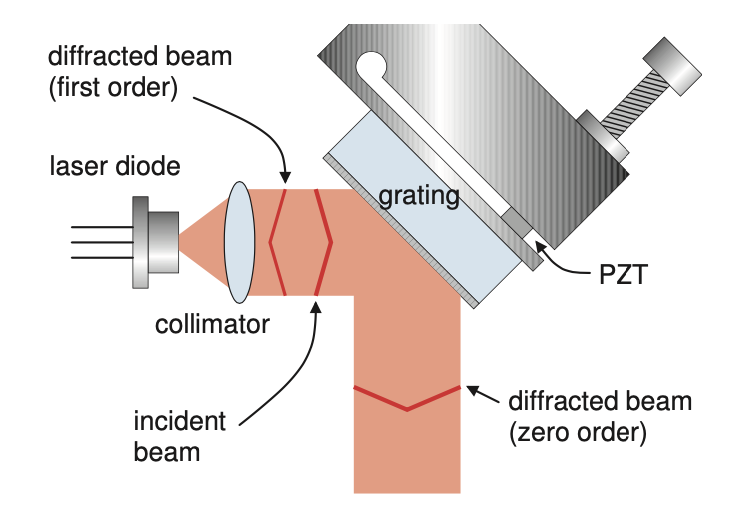
\includegraphics[width=\linewidth]{figs/experimental_setup/pzt.png}
	\caption{Principle schematic of the laser system \cite{manual}\label{fig:laser}}
\end{wrapfigure}
The heart peace of this experiment is the laser (\textbf{L}ight \textbf{A}mplification by \textbf{S}timulated \textbf{E}mission of \textbf{R}adiation). It will be used to set the Rubidium atoms in excited states, s.t. we can do laser spectroscopy. There are different kinds of lasers. The currently most efficient ones are solid state lasers like the used laser system \emph{DLC DL Pro} from Toptica. It is an extended cavity laser with feedback from an external grating mounted in Littrow configuration. It can be controlled via an electronic control unit (ECU). The normal operation wavelength of the laser is $\lambda_0=794$nm with an output power of about 7mW. \cite{manual}

A principle scheme of the laser is given in figure \ref{fig:laser}. The laser consists of a laser diode that emits the light. It gets collimated and falls on a grating element, that is placed on a \emph{piezo-electric transducer} (PZT). By applying a current on the PZT, one can rapitly change the grating angle. On the grating the first beam order gets reflected and acts as an external feedback, while the zero order will be diffracted as the output beam. \cite{manual}

It is our interest to vary the wavelength of the laser. For this we can use different approaches \cite{manual}:
\begin{enumerate}
	\item Laser temperature: The output frequency of a GaAs laser decreases for rising temperatures. This effect comes from the thermal expansion of the crystal and a temperature dependent gain shift. To avoid temperature influences, one has to start the laser in advance, s.t. the temperature is stabilized. This method will not be used for wavelength variation, since this method would be really slow. 
	\item Laser current: With the modification of the laser current gets the refraction index of the gain medium modified. This is the result of changing carrier density and is based in Ohmic heating due to finite quantum efficiency of the device. This internal heating would allow high change rates of a few MHz.
	\item Grating angle: Optical feedback from external diffraction grating is possible in a narrow range of angles. Due to complicated interplay of the gain medium dynamics and optical feedback have those angle modifications impact on the output wavelength. In best case setups, one could get only one resulting laser mode. For more information see e.g. {\cite{grating}}.
\end{enumerate} 
We fixed the laser current such that a stable laser operation on only one mode was ensured (no mode-hopping) and used the grating angle that also triggers the oscilloscope as an external trigger to modify the wavelength. Thus absorption spectra could be observed directly on the oscilloscope.  

\subsection{Fabry-Perot-Interferometer}
We will use the confocal FPI to produce a frequency reference for the atomic spectra. For this experiment we used a FPI consisting of a resonator with two spherical mirrors (mirror radius $r_\text{mirror}=500$m, reflectivity $R(794\text{nm})\approx0.85$) separated by $L=500$mm inside of a quartz tube and mounted on steel rings, s.t. the thermal expansions are compensated. The resonator is encapsuled inside of a brass tube, that is used as a thermal mass. \cite{manual}
 
 In the following we will shortly introduce the most important equations that will be used in the analysis. For more informations and derivations consult a standard optics book like \cite{hecht}. 
 
 One characteristic of the FPI is the periodic resonant transmission of the incoming beam that is given by
 \begin{align}
 	T_{\text{FPI}}=\frac{1}{1+F\sin^2({\varphi/2})} &&\text{with}&&F=\frac{4R}{(1-R)^2}
 \end{align}
where the phase of one round trip can be written as 
$$\frac{\varphi}{2}=nk_0L=\frac{2\pi n L}{\lambda_0}=\frac{n_\omega L}{c}.$$
The free spectral range (FSR) is the frequency space between transmission peaks and defined as
\begin{equation}
	\Delta \nu_{\text{FSR}}=\frac{c}{2nL}
\end{equation}
where $n$ is in our case the refraction index of air $n=n_\text{air}=1$. For highly reflective mirrors is the full width half maximum (FWHM) given in dependence of the finesse $\mathcal{F}$ and the free spectral range (range between two transmission maxima) $\delta\nu_\text{FSR}$ by
\begin{align}
	\Delta\nu_\text{FHWM}=\frac{\delta \nu_\text{FSR}}{\mathcal{F}} &&\text{with}&&\mathcal{F}=\frac{\pi\sqrt{R}}{1-R}
	\label{eq:finesse}
\end{align}
Because the laser may also excite transverse modes (not only longitudinal) the total spectrum of the cavity will have a mode spacing of 
\begin{equation}
	\nu_\text{mode}=\frac{\Delta \nu_{\text{FSR}}}{2}=\frac{c}{4nL}=149.9348(2)MHz
	\label{eq:calib}
\end{equation}
as measured by the \emph{Institut für Angewandte Physik} Bonn. \cite{manual}
\subsection{Optics}
The detailed optic-setups (lenses etc.) we used for the different parts of the experiment will be shown in the next section \ref{sec:anal}, together with measurements and analysis.
\newpage
\section{Measurements and Analysis}
\label{sec:anal}
We show here our measurements and analysis in chronologous order.
\subsection{Diode laser characteristics}
First we measured the laser output power in dependence of the laser current which we expect to be linear once the threshold current $I_\text{thr}$ after which laser emission starts has been reached. We used the setup from figure \ref{fig:linearexp}, we did not use the grating to scan the laser frequency. Our measurements are depicted in figure \ref{fig:linear}. We assumed ten percent error on all power measurements since we lack any other estimate.
\begin{figure}[htbp]
	\centering
	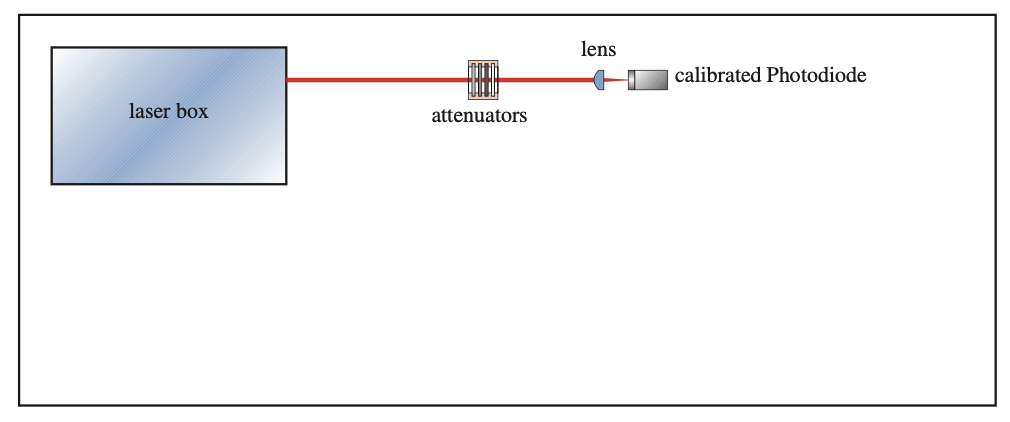
\includegraphics[width=.7\linewidth]{figs/experimental_setup/setup1.png}
	\caption{Setup for measuring the output power $P(I)$\cite{manual}}
	\label{fig:linearexp}
\end{figure}

\begin{figure}[htbp]
	\centering
	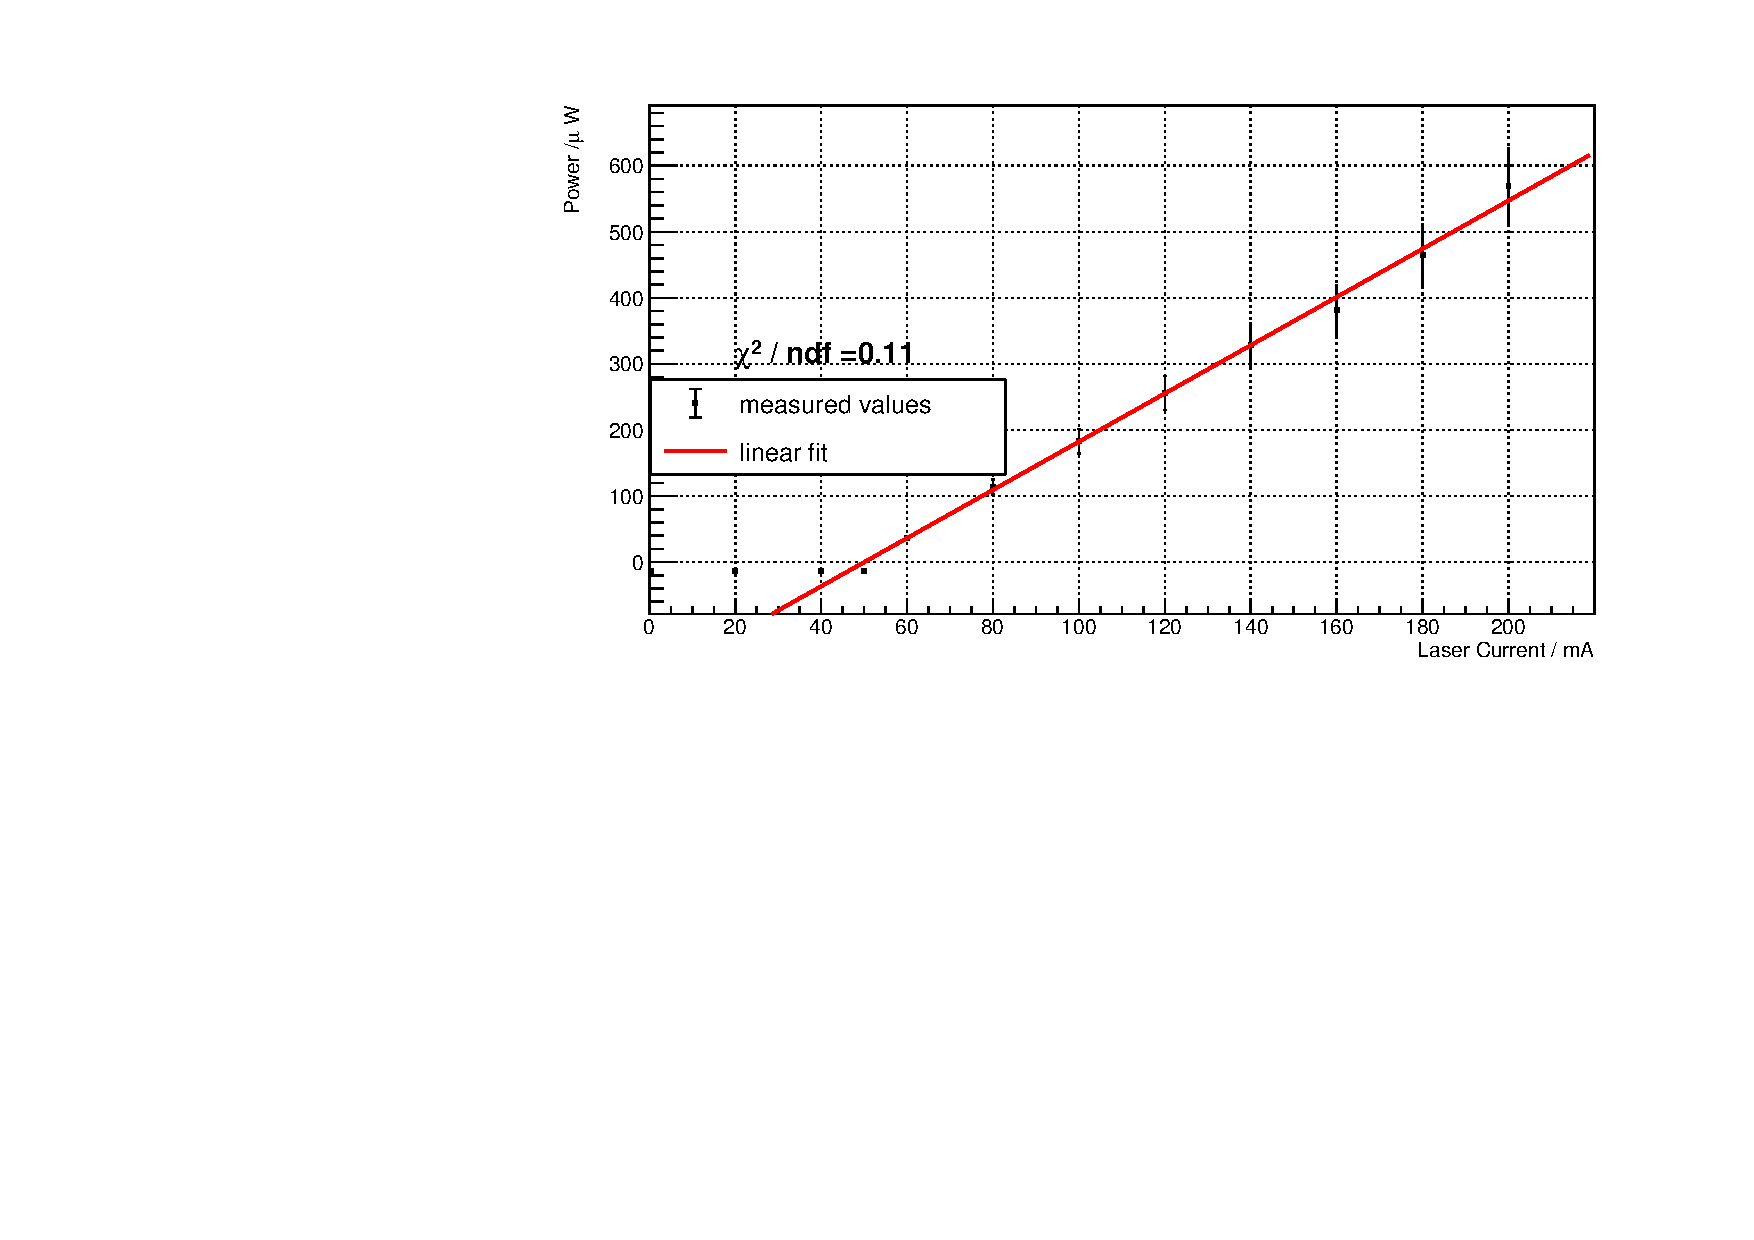
\includegraphics[width=\linewidth]{figs/measurements/laser_current.pdf}
	\caption{Laser power in dependence of laser current}
	\label{fig:linear}
\end{figure}
From the linear fit using ROOT we obtain the fit parameters ($y=mx+n$) \begin{align*}
	m=\SI{3.65\pm0.17}{\micro\W\milli\A^{-1}} && n =   \SI{-182.54\pm11.76}{\micro\W}. 
\end{align*}
Using these results we can calculate the threshold current $$I_{\text{thr}}=-\frac{n}{m}=\SI{50.01\pm3.98}{\milli\A}$$
as well es the \emph{quantum efficiency} Q.E. which is given by the number of generated photons per injected electron  $$\text{Q.E.}=\frac{N_\gamma}{N_e}=\frac{N_\gamma/t}{N_e/t}=\frac{P/E_{\lambda=\SI{794}{\nano\m}}}{I/e}.$$
Table \ref{tab:qe} and figure \ref{fig:qe} show our results for the quantum efficiency depending on the input current. 
\begin{figure}

	
	\centering
	\begin{minipage}{.3\linewidth}
		\centering
		\begin{tabular}{cc}
			\toprule
			Current / mA & Q.E.      \\
			\hline
			60           & $3.843\cdot 10^{-4}$ \\
			80           & $9.126\cdot 10^{-4}$ \\
			100          & $1.172\cdot 10^{-3}$ \\
			120          & $1.366\cdot 10^{-3}$ \\
			140          & $1.505\cdot 10^{-3}$ \\
			160          & $1.525\cdot 10^{-3}$ \\
			180          & $1.654\cdot 10^{-3}$ \\
			200          & $1.825\cdot 10^{-3}$\\
			\bottomrule
		\end{tabular}

	\end{minipage}
	\begin{minipage}{.69\linewidth}
			\centering
			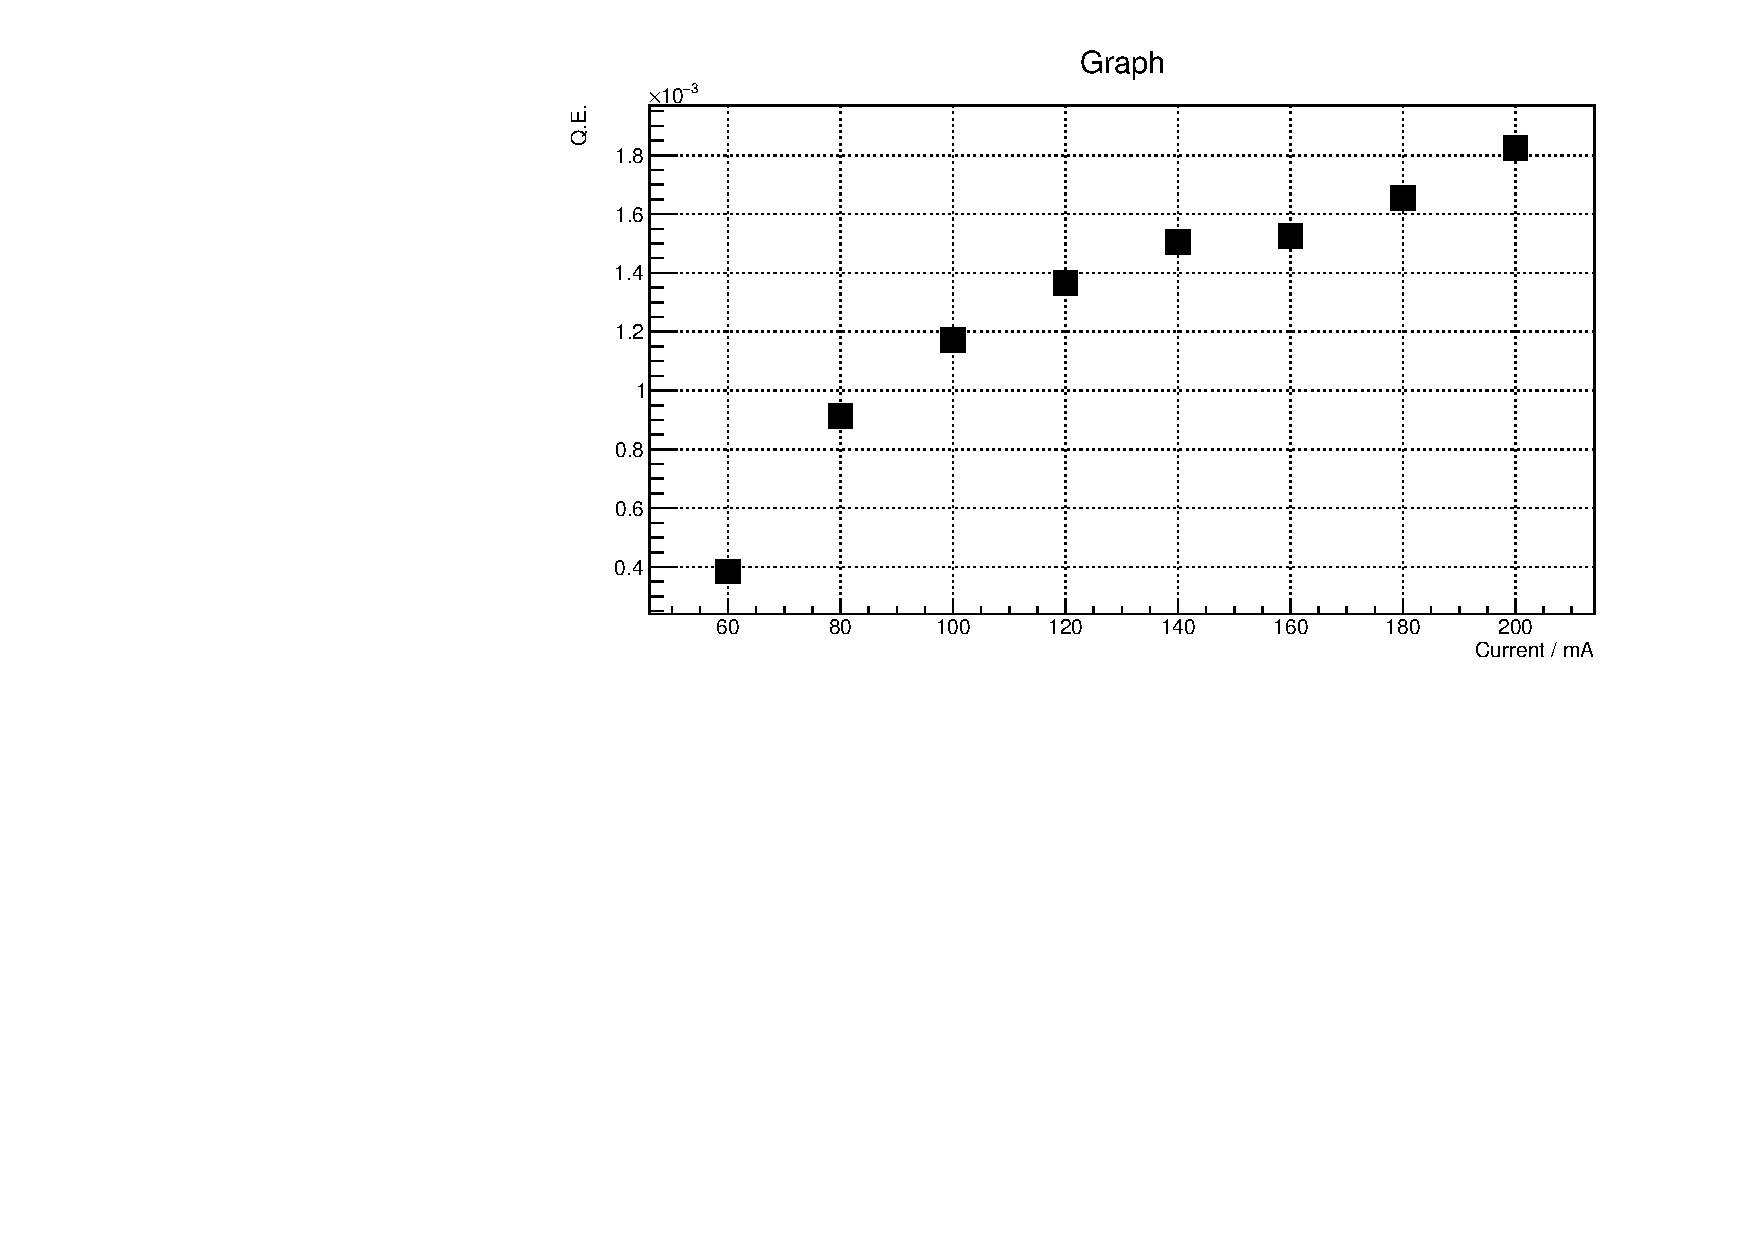
\includegraphics[width=\linewidth]{figs/measurements/qe.pdf}


	\end{minipage}
 \captionlistentry[table]{Quantum efficiency as a function of laser current}
 \label{tab:qe}
\captionsetup{labelformat=andtable}
\caption{Quantum efficiency as a function of laser current}
\label{fig:qe}
\end{figure}



We see our expectations confirmed that only after a certain threshold a linear dependence of the laser power on the laser current holds. Before the threshold there is no measurable power (We ignored the offset of \SI{-13}{\micro\W} since it won't affect the linear fit and we can avoid additional errors). In principle one could also expect a linear dependence of output power \emph{before} laser emission; in this regime the laser diode functions just like an LED \cite{laser}. But since the emission is incoherent and there is significant distance between laser and power meter the measured power is negligible. The quantum efficiency is rather small but one has to consider that the beam is attenuated before measuring the power, thus influencing the result.
\subsection{Use of the Fabry-Perot interferometer}
The next part of our experiment considered the FPI. In figure \ref{fig:FPI} the setup we used is shown. 
\begin{figure}[htbp]
	\centering
	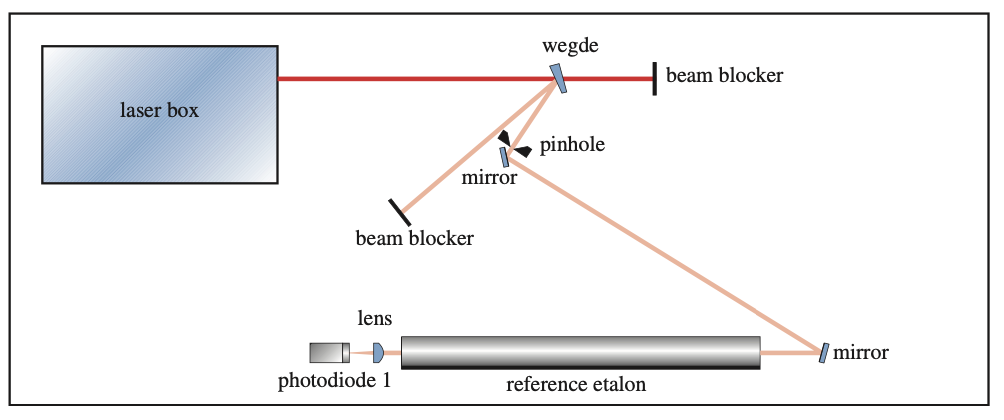
\includegraphics[width=\linewidth]{figs/experimental_setup/setup2.png}
	\caption{Setup for coupling the laser into the FPI \cite{manual}}
	\label{fig:FPI}
\end{figure}

First we use a wedge to split the beam into two weak beams and strong beam. One weak beam and the strong beam are blocked for now. The free beam is guided through a pinhole to avoid backwards reflections into the laser \cite{manual} and coupled into the FPI using two mirrors which provide the necessary degrees of freedom. After the FPI the transmitted intensity is measured on a photodiode and can be observed on the oscilloscope. We scan the laser frequency in order to observe the periodic transmission of the FPI which we can use as a calibration in time later on.

Figure \ref{fig:fpi} shows the first five peaks of the periodic transmission we could observe. Note that the time axis is in relative units to the start of the measurements. The oscilloscope provided us only with the voltage data and we had to calculate the relative time from the beginning of the measurement. The time steps (\texttt{sampling rate}) were $8\cdot10^{-8}$ s.

\begin{figure}[htbp]
	\centering
	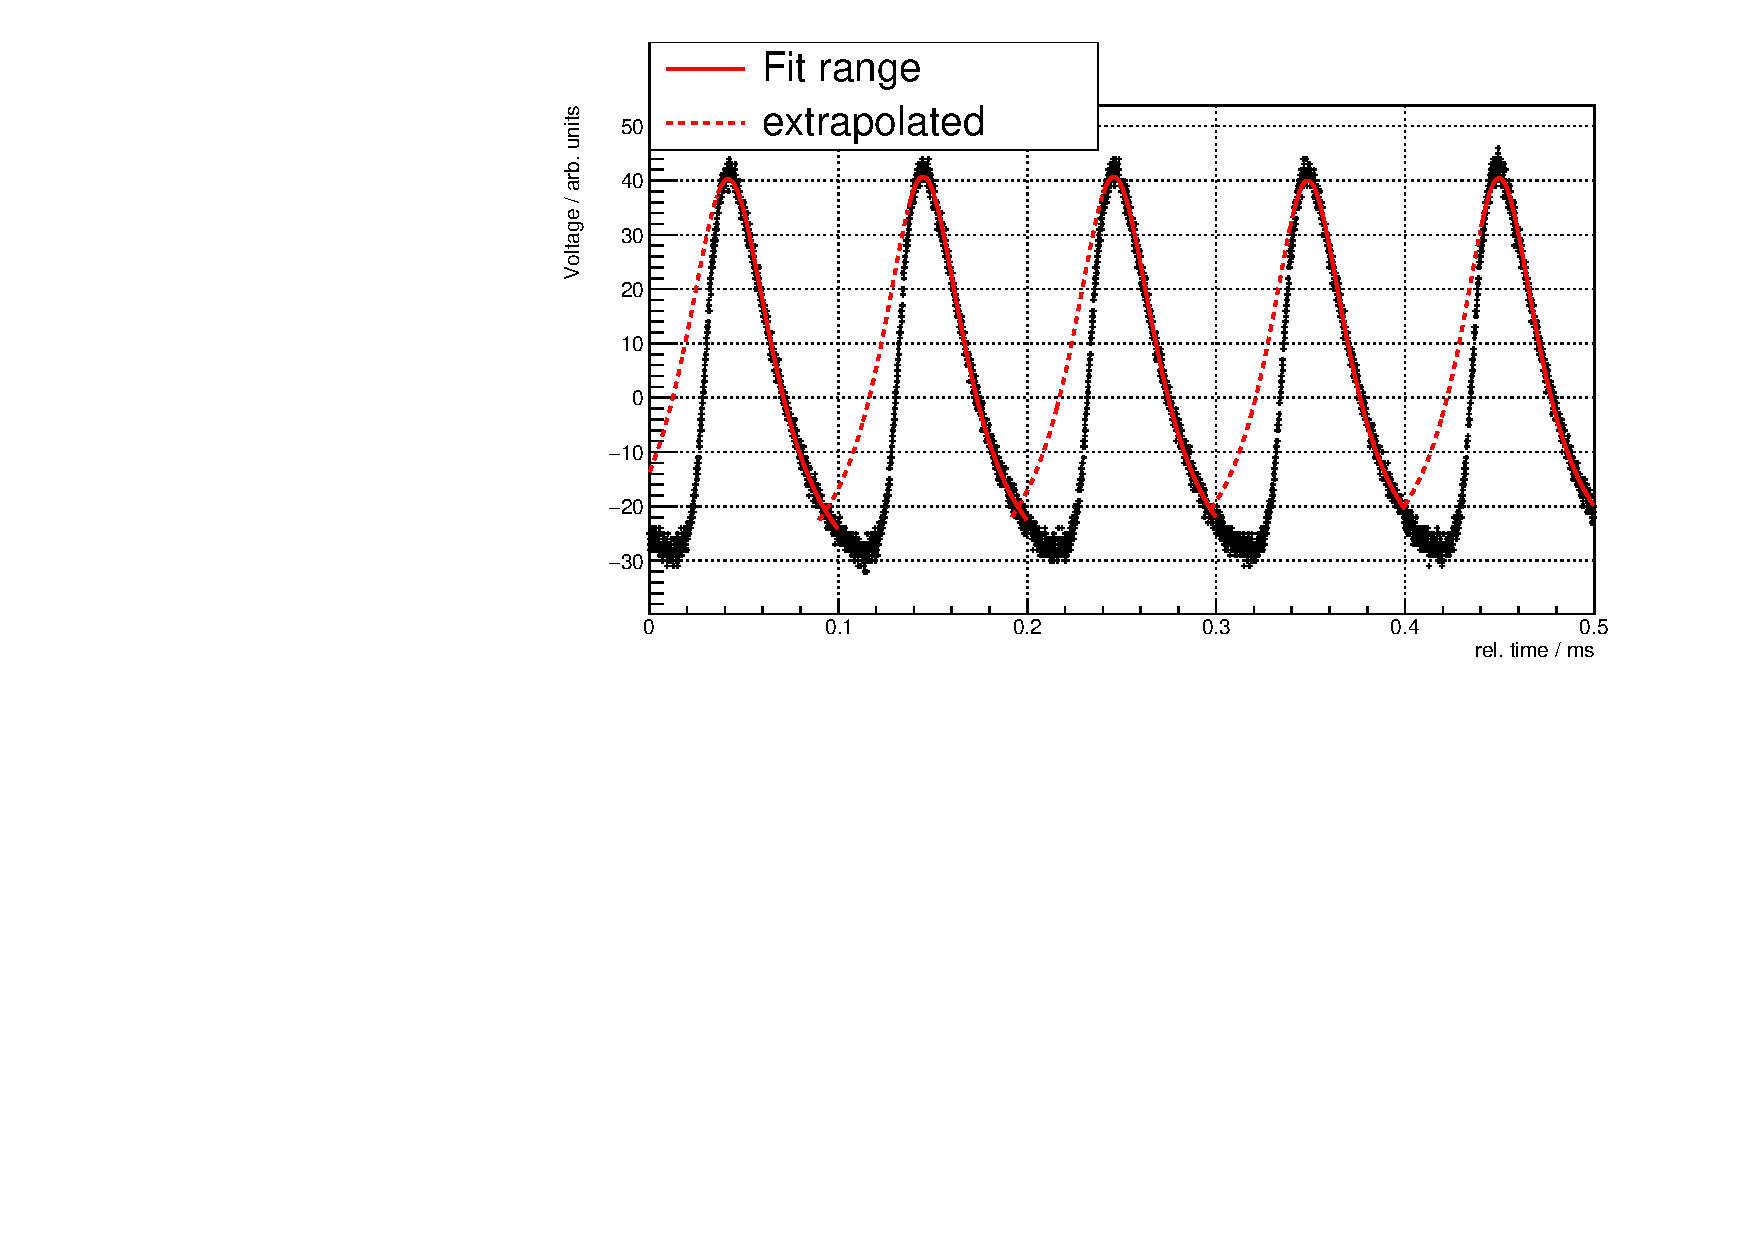
\includegraphics[width=\linewidth]{figs/measurements/fpi.pdf}
	\caption{Periodic transmission of the FPI. We fitted \textsc{Lorentz} functions to the peaks}
	\label{fig:fpi}
\end{figure}

To estimate the peak positions it is evident to fit \textsc{Lorentz} functions to the peaks $$f(x)=A\frac{(\Gamma/2)^2}{(x-x_0)^2+(\Gamma/2)^2}+B,$$
witch peak position $x_0$ and FWHM $\Gamma$.
We observe however that the peaks are not symmetric. This is likely due to the photodiode having different rise and fall times for incoming signals. We thus fitted the peaks with a strong bias to the falling flank because here the function fits the data best (this is only an observation having no theoretical basis whatsoever). From our fits we find a mean FWHM of $$\hat{\Gamma}=(0.05506\pm0.00024)\text{ ms}$$
and a mean distance between two subsequent peaks of $$\Delta t=(0.10202\pm0.00030)\text{ ms}.$$ 
We can now determine the finesse of the FPI using equations \cref{eq:finesse}. We find with a reflectivity of $R=0.85$ \cite{manual}
\begin{align*}
	\mathcal{F}^{theo}=\frac{\pi\sqrt{R}}{1-R}=19.31 && \mathcal{F}^{exp}=\frac{\delta\nu_{\text{FSR}}}{\Delta\nu_\text{FHWM}}=\frac{\Delta t}{\hat{\Gamma}}=1.85\pm0.01. 
\end{align*}
The experimentally determined finesse is a factor of 10 smaller than the theoretically expected value. This can only be explained by a reflectivity which is in fact smaller than the given $R=0.85$. The experimentally determined value coincides with $R\approx0.24$. This on the other hand is much smaller than the nominal value. Another major source for the error will lie in the fact that the transmission peaks could not be fitted as a whole because of their asymmetric form. This in turn could have lead to an overestimation of the FWHM.

Using equation \eqref{eq:calib} we can estimate a calibration which relates time intervals to frequency intervals, namely $$\Delta[\si{\mega\Hz}]=c\cdot\Delta[\si{\milli\s}],$$ with $$c=\SI{2.9393\pm0.0086}{10^3\mega\Hz \milli\s^{-1}}.$$
Now we can evaluate the now following absorption spectra and determine the linewidth of spectral lines easily.






\subsection{Linear spectroscopy of the $D_1$ transition of Rb}
Having prepared the time calibration we can finally measure absorption spectra and analyze them accordingly. Figure \ref{fig:linearspec} shows the setup we used.
\begin{figure}[htbp]
	\centering
	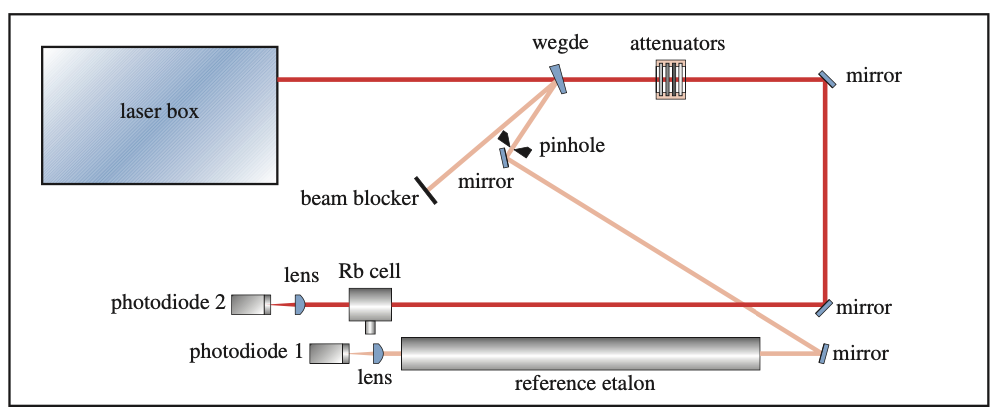
\includegraphics[width=\linewidth]{figs/experimental_setup/setup3.png}
	\caption{Experimental setup for linear absorption spectroscopy\cite{manual}}
	\label{fig:linearspec}
\end{figure}
The setup basically just extends the one we used to measure the finesse of the FPI by coupling the strong laser beam we blocked before into a cell with Rb vapor (length 5 cm) and a photodiode afterwards. The laser frequency is again scanned using the grating, allowing us to measure the hyperfine absorption spectrum exactly. With the calibration done before we can determine frequency intervals from time intervals. We do not have to make the time-frequency calibration again since we did not alter any parameters in the FPI optics. Still we observe the FPI output to be sure we are operating the laser stable.  Figure \ref{fig:linearfit} shows an absorption spectrum with fits to the peaks. The time steps are given by $8\cdot10^{-7}$ s.
\begin{figure}[htbp]
	\centering
	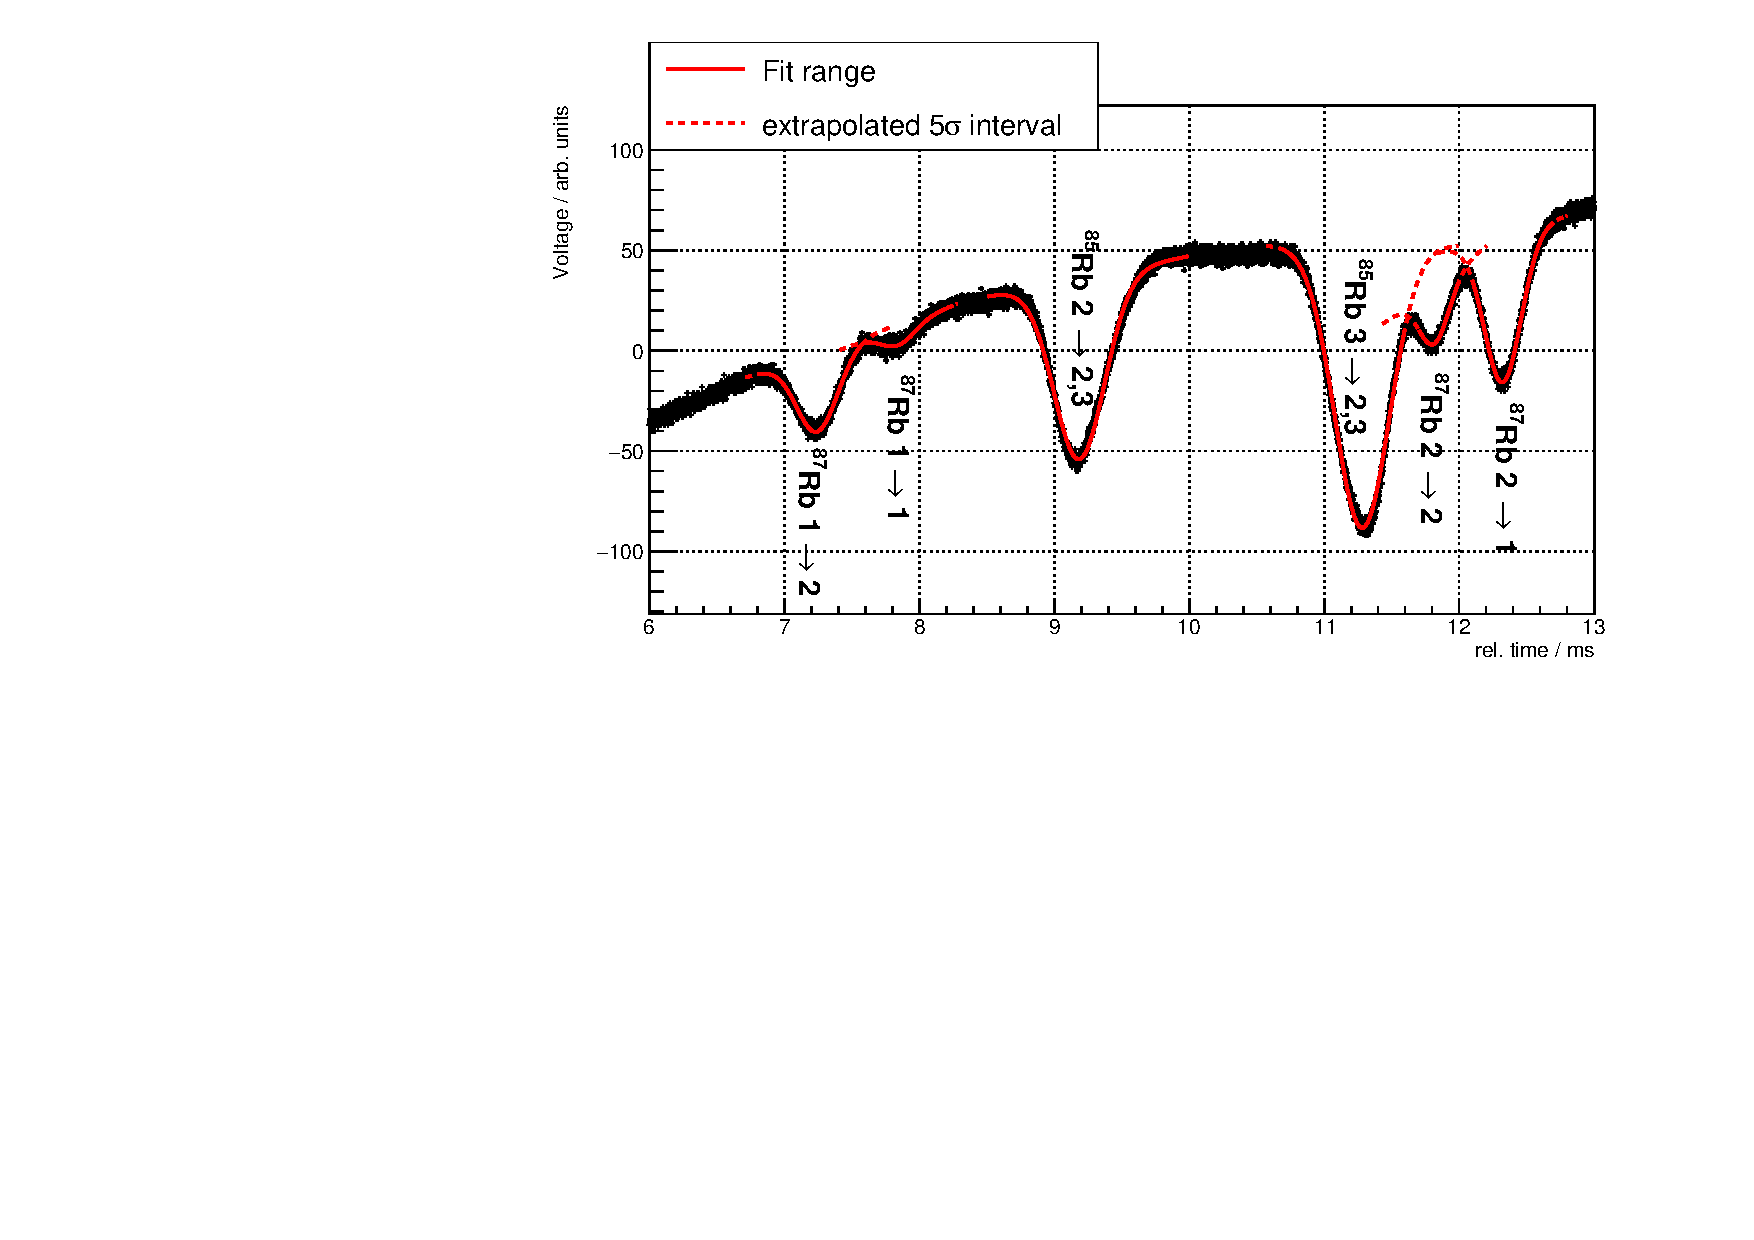
\includegraphics[width=\linewidth]{figs/measurements/linear.pdf}
	\caption{Absorption spectrum recorded with the 5 cm vapor cell. $i\to j $ indicates the transition from $F=i$ to $F=j$, , frequency is decreasing from left to right.}
	\label{fig:linearfit}
\end{figure}
We notice that the output power is not completely independent of the grating angle (or laser frequency) as can be seen by the approximately linearly rising noise which is only constant in a small frequency region. Using the transition probabilities in figure \ref{fig:hfs} we can identify the two most prominent lines as $^{85}$ Rb lines where the most intense one must be the transition $F=2\to2,3$ meaning that the frequency decreases from left to right. With this information all other lines can be mapped to the spectrum easily. This also means that the hyperfine splitting in the excited state of $^{85}$ Rb cannot be resolved with this setup. To determine the peak positions, widths and amplitudes we fitted \textsc{Gaussian} functions with linear background to the data 
$$f(x)=A\exp\left[\frac{(x-x_0)^2}{2\sigma^2}\right]+C\cdot x +D,$$
because the lines are \textsc{Doppler} broadened.

\subsubsection{Hyperfine splitting}
We can now determine the hyperfine splitting constant $A_\text{HFS}$ for the ground states and for $^{87}$Rb also the excited state can be investigated.

\paragraph{\boldmath{$^{85}$}Rb}
Let us first consider what the splitting should theoretically be. The $5S_{1/2}$ state splits into two substates with (see \eqref{eq:hfs}) $$\Delta E_\text{HFS}=\begin{cases}
	\phantom{-}5/2A_\text{HFS} & F=3\\
	-7/2A_\text{HFS} & F=2
\end{cases}.$$
This means the splitting of the ground state is given by $$\Delta E_S ^{85}=6A_\text{HFS}.$$
The separation of the two $^{85}$Rb line is $$\Delta t = \SI{2.0957\pm0.0006}{\milli\s}. $$ Thus $$ A_{5S_{1/2}}=h \cdot c\cdot\Delta t/6=h \cdot \SI{1026.6387\pm3.0179}{\mega\Hz}.$$
This is near the literature value \cite{85d} of $$A_{5S_{1/2}}=h \cdot \SI{1011.9108130\pm0.0000020}{\mega\Hz},$$ the relative error is $1.16\%$. The absolute deviation is within $4\sigma$.


\paragraph{\boldmath{$^{87}$}Rb}
The ground and excited state splits like 
$$\Delta E_\text{HFS} (5S_{1/2})=\begin{cases}
	\phantom{-}3/2A_\text{HFS} & F=2\\
	-5/2A_\text{HFS} & F=1
\end{cases}.$$
This means the splitting of ground and excited state is given by
$$\Delta E_{S/P} ^{87}=4A_{\text{HFS},S/P}.$$
The mean of the separation between the two lower levels is $$\Delta t = \SI{4.5252\pm0.0079}{\milli\s} $$

 Thus $$ A_{5S_{1/2}}=h \cdot c\cdot\Delta t/4=h \cdot \SI{3325.2524\pm11.3402}{\mega\Hz}.$$
 This is near the literature value \cite{87d} of $$A_{5S_{1/2}}=h \cdot \SI{3417.34130545215\pm0.00000000002}{\mega\Hz},$$ the relative error is $2.70\%$. The absolute deviation is within $8\sigma$.
 
 The mean of the separation between the two upper levels is $$\Delta t=\SI{0.5534\pm0.0079}{\milli\s}.$$
  Thus $$ A_{5P_{1/2}}=h \cdot c\cdot\Delta t/4=h \cdot \SI{406.6480\pm5.9461}{\mega\Hz}.$$
 This is near the literature value \cite{87d} of$$A_{5P_{1/2}}=h \cdot \SI{408.328\pm0.015}{\mega\Hz},$$ the relative error is $0.4\%$. The absolute deviation is within $1\sigma$.
 
 Table \ref{tab:hfs} summarizes our findings.
 \begin{table}[htbp]
 	\centering
 	\begin{tabular}{c|c|c}
 		\toprule
 		energy level & $A_\text{HFS} \cdot h / \si{\mega \Hz} $ & rel. error \\
 		\hline
 		$5S_{1/2}(^{85}\text{Rb})$& $ 1026.6387\pm3.0179$& $1.16\%$\\
 		$5S_{1/2}(^{87}\text{Rb})$& $ 3325.2524\pm11.3402$& $2.70\%$\\
 		$5P_{1/2}(^{87}\text{Rb})$& $ 406.6480\pm5.9461$& $0.4\%$\\
 		\bottomrule
 	\end{tabular}
 \caption{Different hyperfine structure constants determined from the \textsc{Doppler} broadened absorption spectrum.}
\label{tab:hfs} 
\end{table}
 
 It is evident that in small frequency regions we are able to reproduce literature values quite exactly but not in more extended frequency intervals. This may be due to the aforementioned correlation between output power and output frequency which could then influence the goodness of the fits. Nevertheless we can reproduce the order of magnitude for the hyperfine structure constants very good. We do not arrive at the literature values within a statistical error, which means some systematic uncertainties have to be taken into account: the laser output frequency is not independent of output power, this makes the fitting procedure more complicated giving rise to a series of possible systematic errors like the choosing of the actual background function, fit range, etc. Also, the setup could of course have been perturbed by unwanted vibrations caused by the clumsy experimentalist. Having many mirrors installed this can of course alter the course of the laser beam and influence the transmission intensity in FPI and vapor cell only by having angular displacement. As a last possible error source let us mention the time calibration: we assumed our calibration made in the beginning holds for all subsequent measurements since we did not consciously tweak the FPI optics. Nevertheless the optics could have changed over time, making new calibrations necessary for every measurement. General improvement of results could also be reached by using longer vapor cells. This will make the absorption very clear against background and result in easier to fit spectra.
\subsubsection{Spectral resolution}
The smallest measured frequency difference $\Delta\nu$ is between the excited $^{87}$Rb states $$\Delta\nu=\SI{1767.1365\pm14.6410}{\mega\Hz}$$ which leads to a spectral resolution $$\frac{\Delta \nu}{\nu}=(4.6802\pm0.039)\cdot10^{-6}.$$

 
\subsubsection{\textsc{Doppler} width}
We now wish to compare the FWHM of the most prominent line to the \textsc{Doppler} width (eq. \eqref{eq:dopp}). We find a FWHM of $$\Delta\nu_\text{FWHM}=\SI{992.4383\pm3.0840}{\mega\Hz}.$$
Equation \eqref{eq:dopp} predicts a linewidth of (assume $T=\SI{300}{\K}$, $m_\text{atom}=\SI{1.409 993 199e-25}{\kilo\g}$ \cite{85})
$$\Delta\nu_\text{\textsc{Doppler}}=\SI{215.86}{\mega\Hz}.$$
Since this is significantly smaller than our estimate of the FWHM other line broadening effects (collisional broadening, power broadening, saturation broadening \cite{demtröderl}) have to be taken into account to explain this width and not only the \textsc{Doppler} width.
\subsubsection{\textsc{Lambert-Beer} absorption law}
Lastly we want to investigate the law of \textsc{Lambert-Beer} which states that the absorption should increase linearly ($A=1-T$) with the length of the absorber for optically thin media (eq. \eqref{eq:beer}). We can do this by replacing the 5 cm vapor cell with a cell that is only 2 cm long. Looking at figures \cref{fig:beer1,fig:beer2} we can check that eq. \eqref{eq:beer} holds true. Here we compared the amplitudes of the peaks that we were able to fit as a measure of absorption. However it is not really sufficient to look at a data sample consisting of two data points and make any scientific statement. Note that for the shorter vapor cell the two weakest lines are not significant against the background and could not be identified.
\begin{figure}[H]
	\centering
	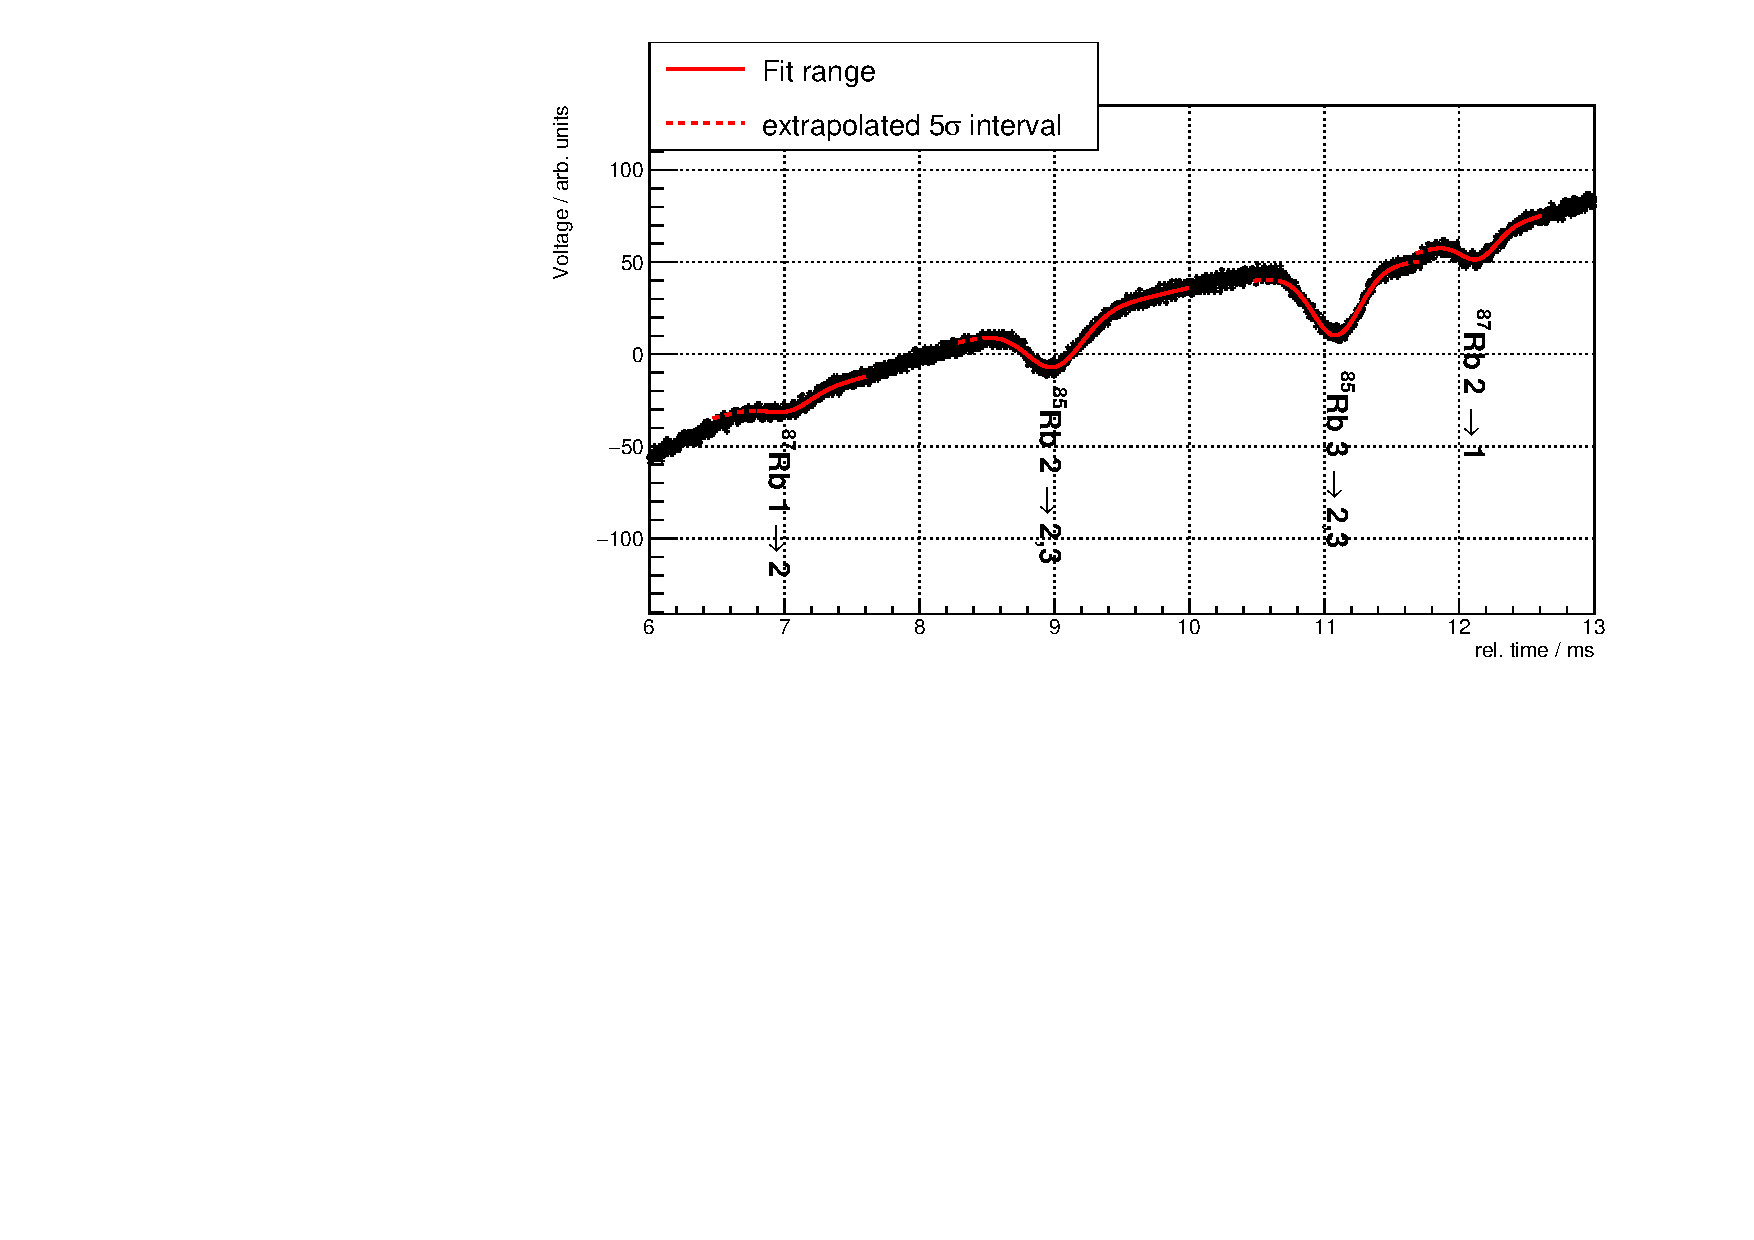
\includegraphics[width=\linewidth]{figs/measurements/short.pdf}

	\caption{Absorption spectrum (frequency is decreasing from left to right) of the shorter vapor cell}
	\label{fig:beer1}
\end{figure}

\begin{figure}[H]
	\centering
	
	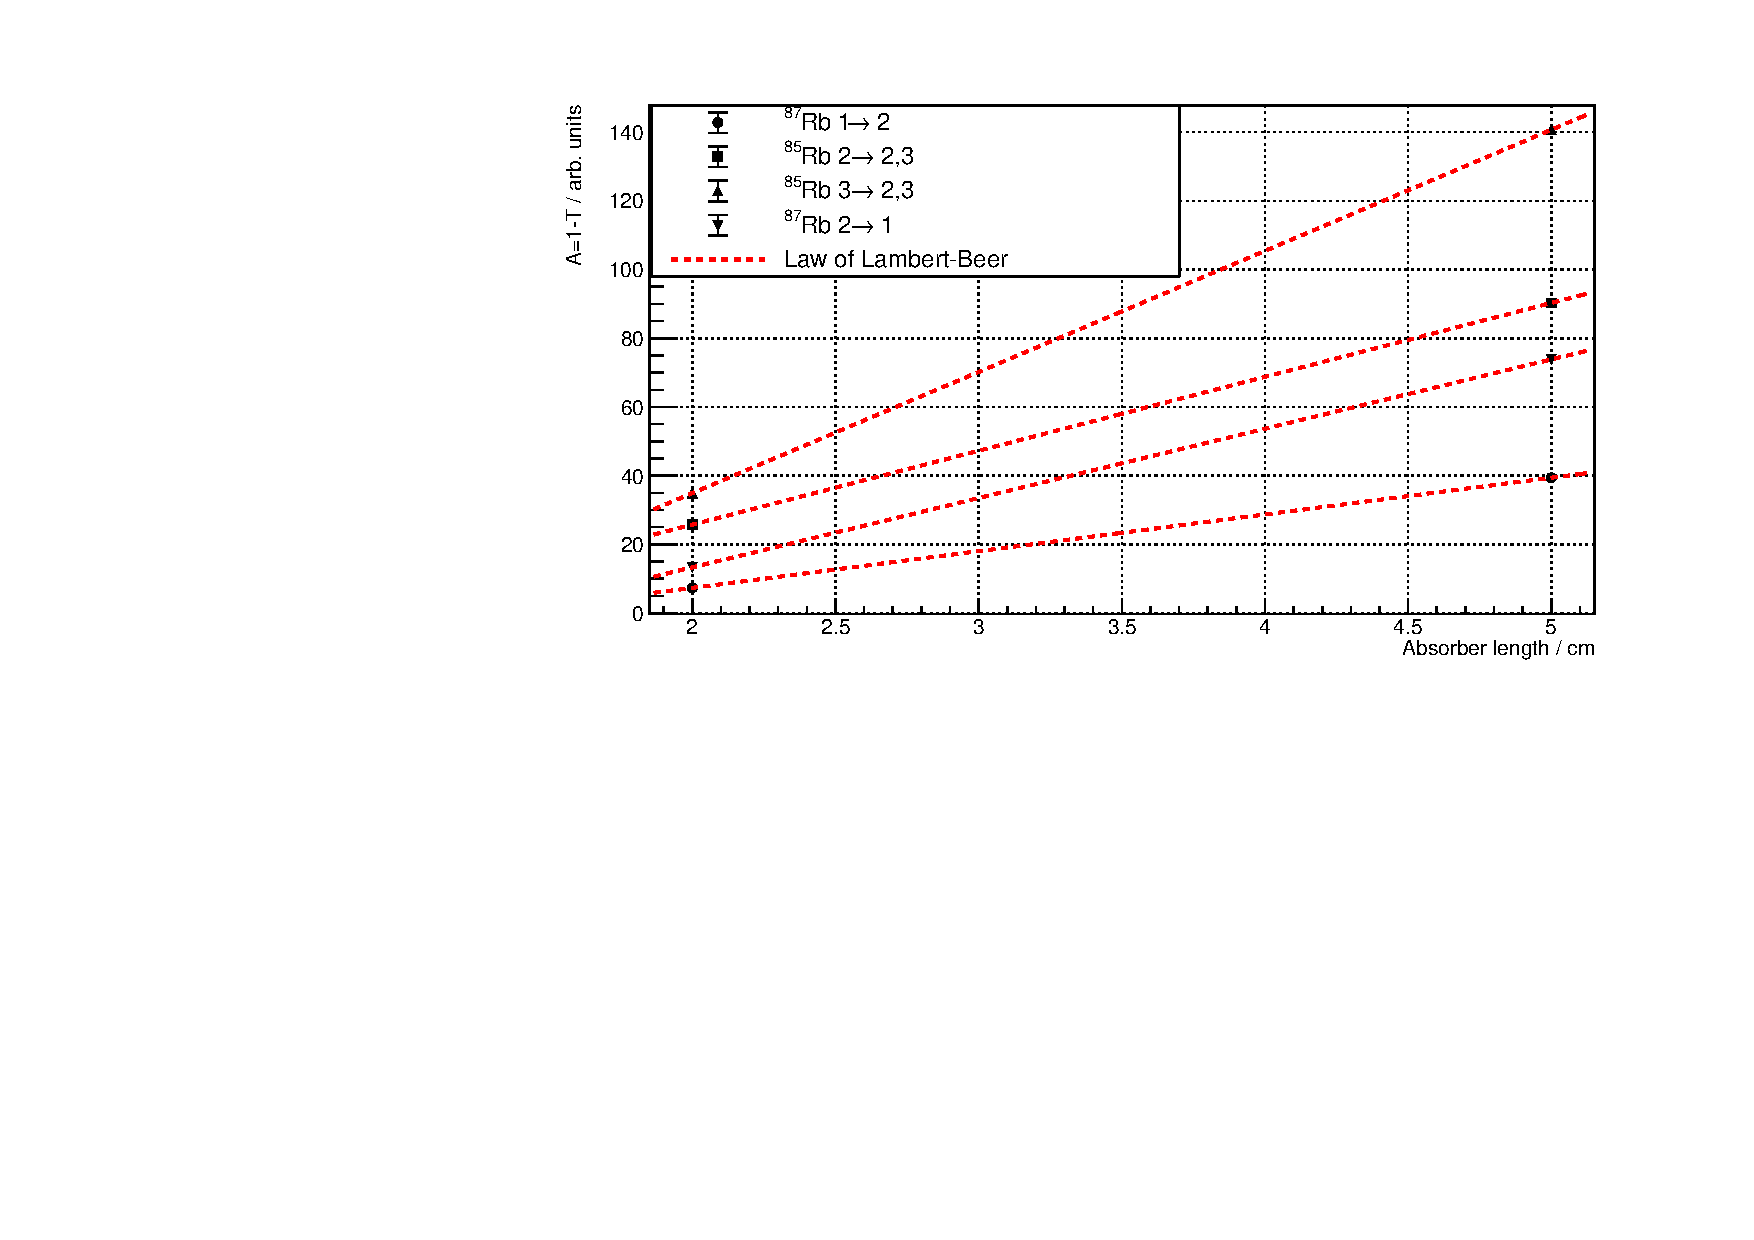
\includegraphics[width=\linewidth]{figs/measurements/beer.pdf}
	\caption{Absorption as a function of cell length.}
	\label{fig:beer2}
\end{figure}

\subsection{Non-linear spectroscopy of the $D_1$ transition of Rb}
We now want to measure the \textsc{Doppler} free absorption spectrum of Rb. For this we prepare a saturated absorption spectroscopy setup, as was explained in section \ref{sec:theory}. Figure \ref{fig:nonlinear} shows the setup we used. 
\begin{figure}[H]
	\centering
	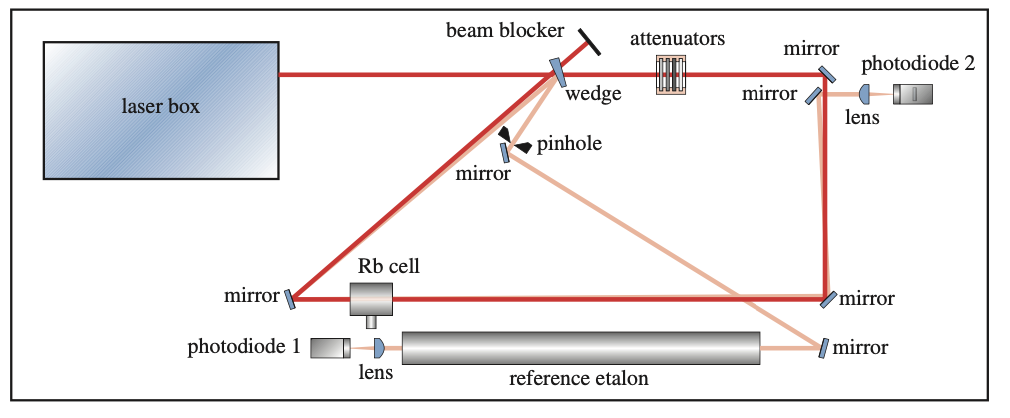
\includegraphics[width=.9\linewidth]{figs/experimental_setup/setup4.png}
	\caption{Setup for non linear absorption spectroscopy\cite{manual}}
	\label{fig:nonlinear}
\end{figure}
It extends the setup from before by employing the before unused weak beam as probe beam. The strong beam functions as saturating pump beam. The absorption spectrum is now measured via the probe beam which is guided into a photodiode over mirrors while the laser frequency is scanned. The calibration from before still holds since we did not alter any parameters in the FPI optics. We still use it to verify we are in stable operation of the laser. Figure \ref{fig:nonlinearfit} shows an absorption spectrum with fits to the peaks. The time steps are given by $8\cdot10^{-7}$ s.

\begin{figure}[H]
	\centering
	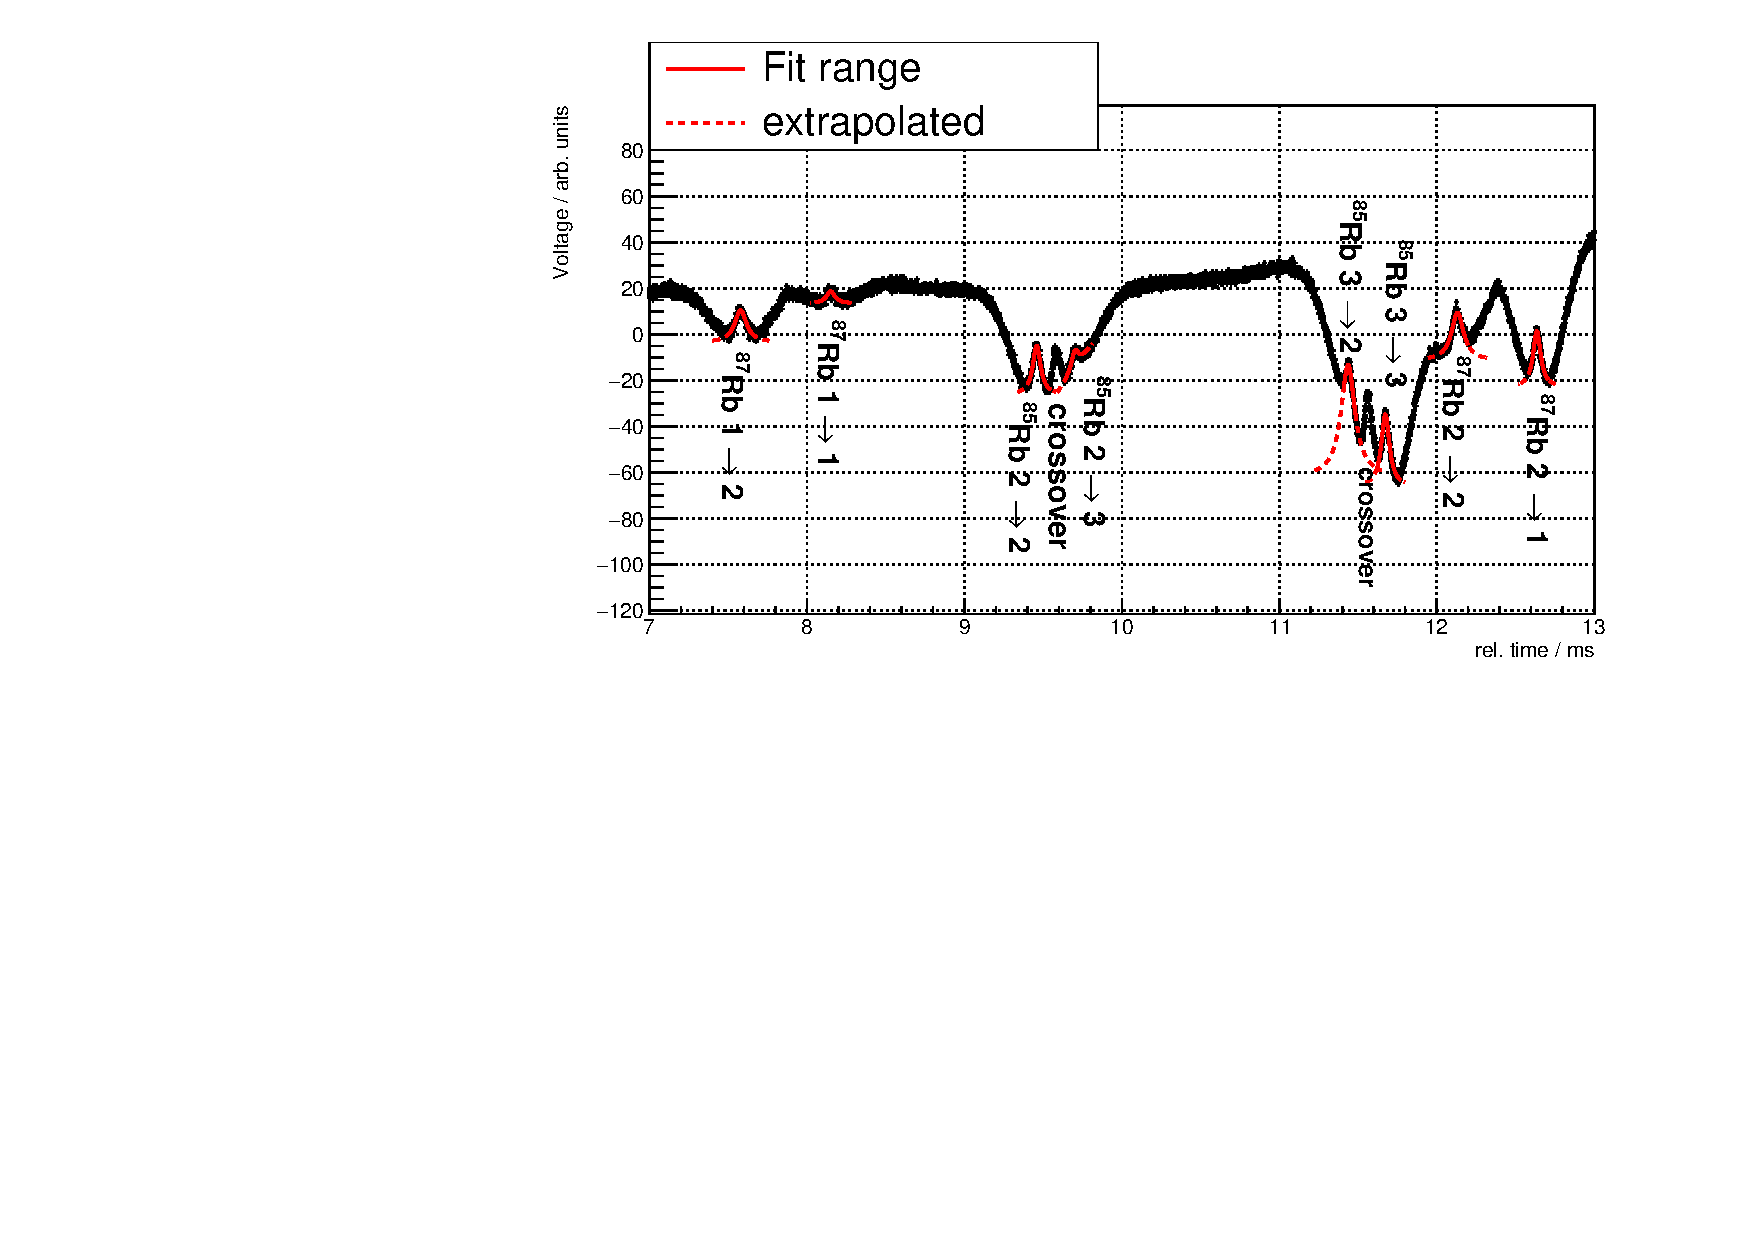
\includegraphics[width=\linewidth]{figs/measurements/nonlinear.pdf}
	\caption{Saturated absorption spectrum of Rb, frequency is decreasing from left to right.}
	\label{fig:nonlinearfit}
\end{figure}

To fit the \textsc{Doppler} free peaks we used \textsc{Lorentzian} line profiles with linear background (where necessary) $$f(x)=A\frac{(\Gamma/2)^2}{(x-x_0)^2+(\Gamma/2)^2}+B\cdot x + C.$$

\subsubsection{Hyperfine splitting}
Again, we can calculate the hyperfine structure constant $A_\text{HFS}$ now that we know the position of the peaks.
\paragraph{\boldmath{$^{85}$Rb}}
As before $$\Delta E_{S/P} ^{85}=6A_{\text{HFS},S/P}.$$
Using the same steps as before we find for the ground state a mean of $$A_{5S_{1/2}}=h\cdot\SI{967.3077\pm2.8488}{\mega\Hz},$$ with a relative error of $4.4\%$ and an absolute error of $16\sigma$. 
We now find for the first time for the excited state 
$$A_{5P_{1/2}}=h\cdot\SI{117.5109\pm0.4756}{\mega\Hz}.$$
The literature value is \cite{85d} $$A_{5P_{1/2}}=h\cdot\SI{120.527(56)}{\mega\Hz}$$
giving rise to an relative error of $2.5\%$ and an absolute error of $6\sigma$.
\paragraph{\boldmath{$^{87}$Rb}}
As before $$\Delta E_{S/P} ^{85}=4A_{\text{HFS},S/P}.$$
Using the same steps as before we find for the ground state a mean of $$A_{5S_{1/2}}=h\cdot\SI{3320.8825\pm 9.7260}{\mega\Hz}$$ with relative error of $2.8\%$ and an absolute error of $10\sigma$.
And now for the second time for the excited state 
$$A_{5P_{1/2}}=h\cdot\SI{395.3323\pm1.3408}{\mega\Hz}$$ with relative error of $3.18\%$ and absolute deviation of $10\sigma$. Table \ref{tab:hfs1} summarizes our results.
\begin{table}[htbp]
	\centering
	\begin{tabular}{c|c|c}
		\toprule
		energy level & $A_\text{HFS} \cdot h / \si{\mega \Hz} $ & rel. error \\
		\hline
		$5S_{1/2}(^{85}\text{Rb})$& $ 967.3077\pm2.8488$& $4.4\%$\\
		$5P_{1/2}(^{85}\text{Rb})$& $ 117.5109\pm0.4756$& $2.5\%$\\
		$5S_{1/2}(^{87}\text{Rb})$& $ 3320.8825\pm 9.7260$& $2.8\%$\\
		$5P_{1/2}(^{87}\text{Rb})$& $ 395.3323\pm1.3408$& $3.2\%$\\
		\bottomrule
	\end{tabular}
	\caption{Different hyperfine structure constants determined from the \textsc{Doppler} broadened absorption spectrum.}
	\label{tab:hfs1} 
\end{table}
We are again able to reproduce the right order of magnitude for the hyperfine coupling constants. As a whole our results are not as precise as before. This is probably due to the saturation peaks being very shallow. If a stronger pump beam would have been used the peaks would have had more significance against the background. As a consequence the fitting would have yielded more precise results. The general remarks about systematic errors from before can be made again at this point with one addition; the biggest possible overlap of pump beam and probe beam is crucial for this experiment. More overlap will give rise to a clearer spectrum which is less smeared out. As vibrations influence the whole setup, this part of the setup is especially vulnerable.
\subsubsection{Spectral resolution}
The smallest possible frequency difference measured is the one of the excited $^{85}Rb$ state. The mean of the separation is $$\Delta\nu=\SI{705.0654\pm2.8533}{\mega\Hz},$$
such that $$\frac{\Delta\nu}{\nu}=(1.8674\pm0.0076)\cdot10^{-6}.$$
This spectral is as expected better than the resolution of non \textsc{Doppler} free spectroscopy. The improvement in spectral resolution gained by saturation spectroscopy is a factor of $\approx 2.5$ which is remarkable.
\subsubsection{Power broadening}
As a last task we want to measure the power dependence of amplitude and width of the line $5S_{1/2}(F=2)\to5P_{1/2}(F=1)$ of $^{87}$Rb (rightmost line in all previously shown spectra) in order to determine the saturation power/intensity. We alter the power of the laser by placing attenuators in the beam line. Without attenuation the output power was \SI{1560}{\micro\W}. We can calculate the power values using the percentage that is transmitted trough the attenuators: $51.2\%,31.2\%$ and $3.7\%$. We stack all different combinations possible in the attenuator rack which leads to the possible power values in table \ref{tab:power}.

\begin{table}
	\centering
	\begin{tabular}{l|c}
		\toprule
		Attenuators $a_1\cdot a_2\cdot a_3 $& Power / $\si{\micro W} = a_1\cdot a_2\cdot a_3 \cdot \SI{1560}{\micro\W}$\\
		\hline
		$0.512\cdot0.321\cdot0.037$ & 9.49\\
		$0.321\cdot0.037$ & 18.53\\
		$0.037$ & 57.72\\
		$0.512\cdot0.321$ & 256.39\\
		$0.321$ & 500.67\\
		$0.512$ & 798.72\\
		- & 1560\\	
		\bottomrule	
	\end{tabular}
\caption{Possible power measurements}
\label{tab:power}
\end{table}
We measure the amplitude of the peak on the oscilloscope, which is why we assign generous errors based on the scale. The width of the peaks is determined by fitting a \textsc{Lorentzian} as before to the data, extracting the FWHM $\Gamma$. This is shown in figure \ref{fig:widthpower} in the appendix.





Figures \cref{fig:b1,fig:b2} show the dependence of amplitude and width of the line on the pump power. The function fitted on the dependence of width on power is (see eq. \eqref{eq:powernu}) $$\Delta\nu=\Delta\nu\sqrt{1+P/P_\text{sat}}.$$
The dependence of amplitude can be modeled by \eqref{eq:power} $$\text{Amp}(P)=B\frac{P/P_\text{sat}}{\sqrt{1+P/P_\text{sat}}}+C$$
since the amplitude is a measure for the absorbed power. 



\begin{figure}[H]	
	\centering
	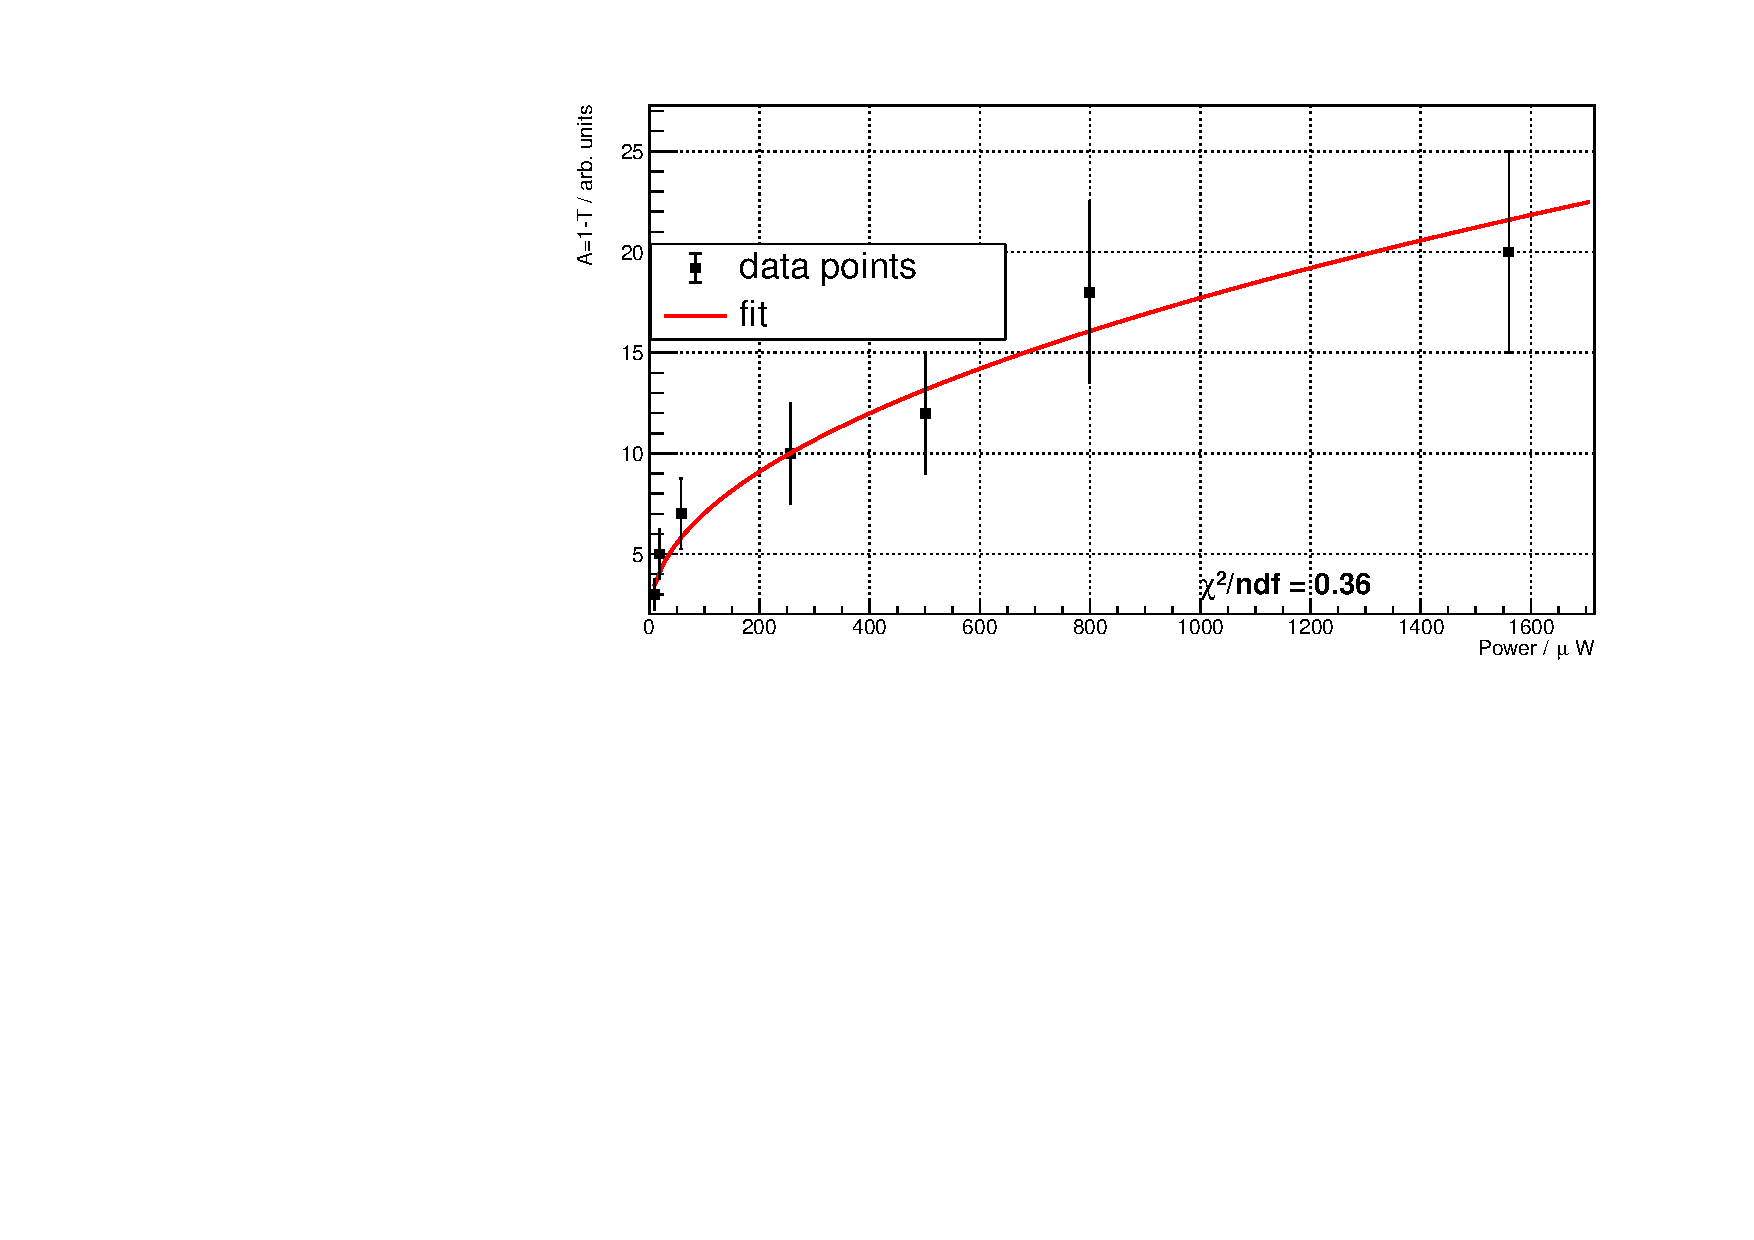
\includegraphics[width=\linewidth]{measurements/amps}
	\caption{Amplitude as function of laser power}
	\label{fig:b1}
\end{figure} 
\begin{figure}[H]	
	\centering
	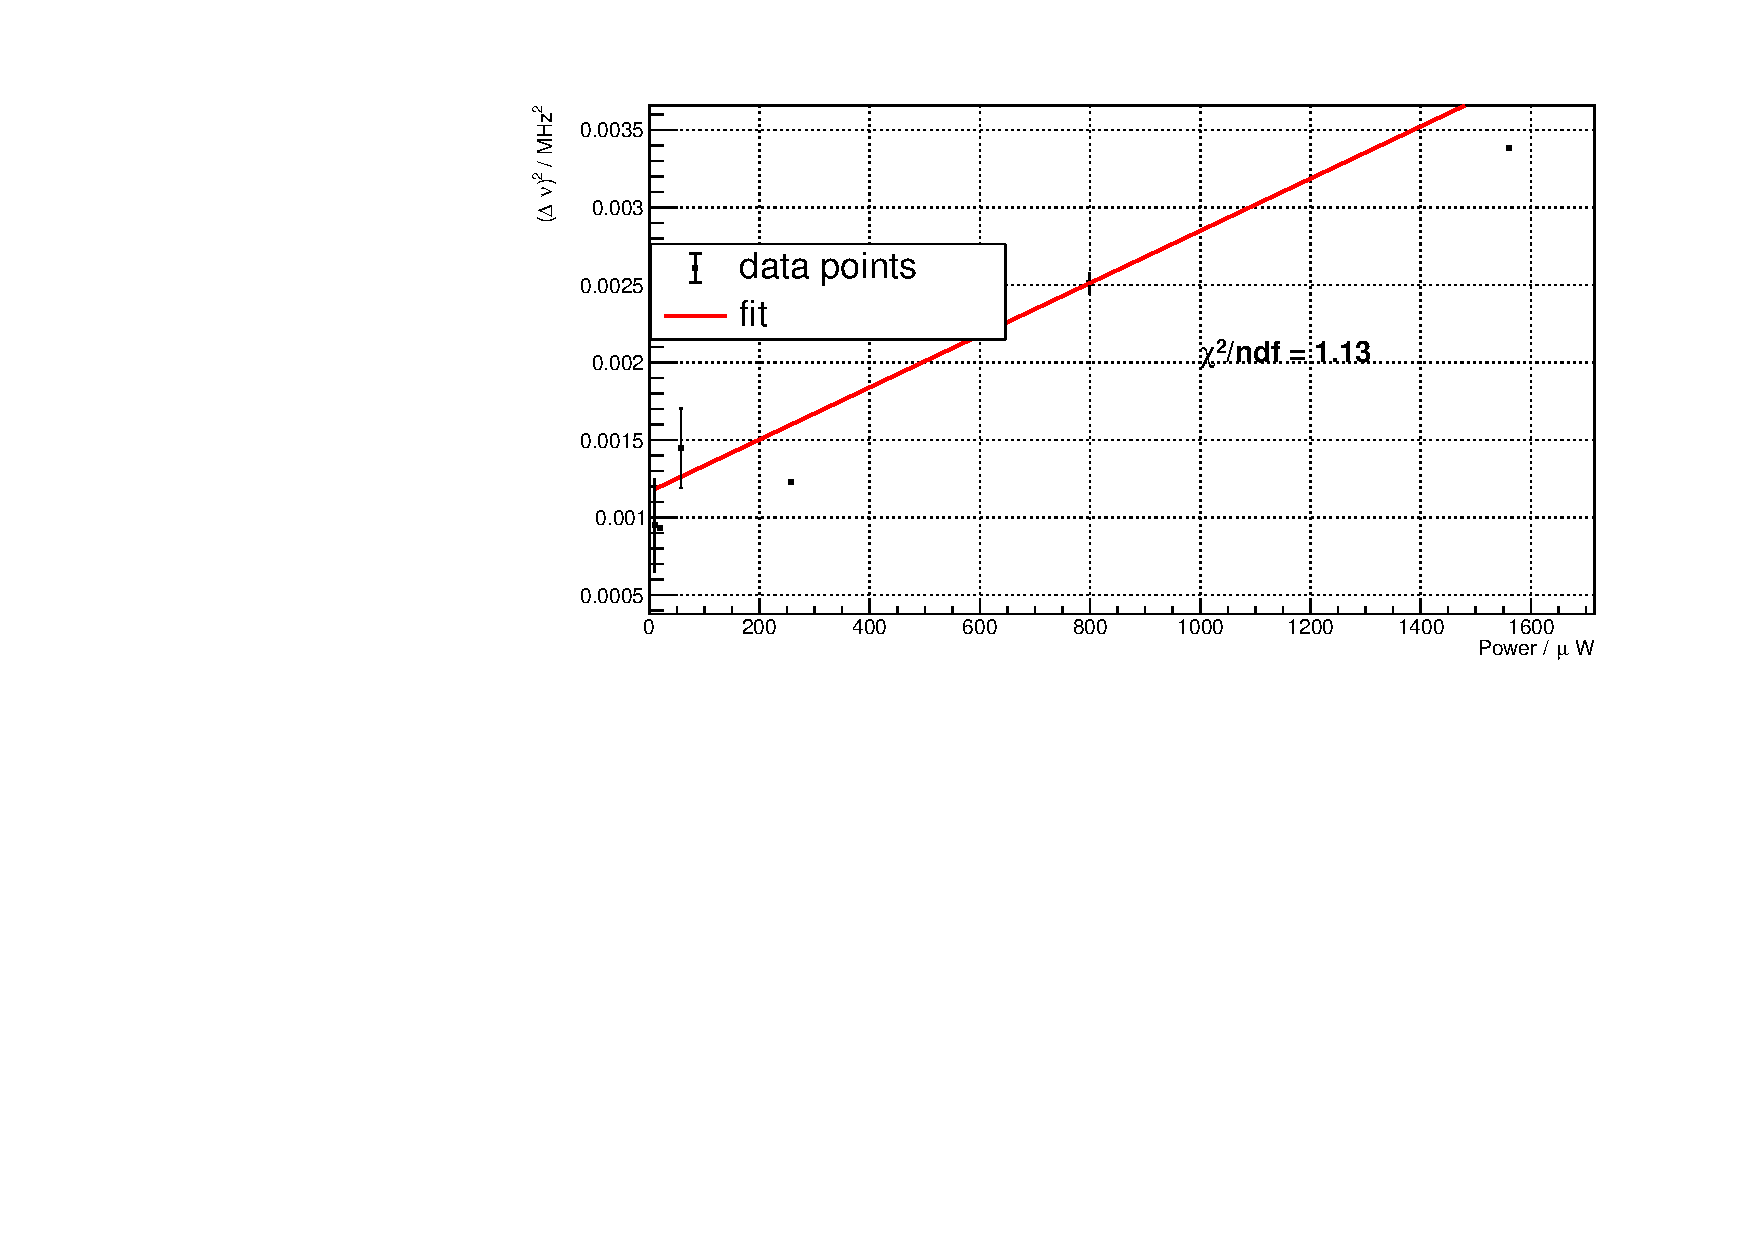
\includegraphics[width=\linewidth]{measurements/widths_fit}
	\caption{FWHM$^2$ as function of laser power, errors at some points too small to be seen}
	\label{fig:b2}
\end{figure} 
From the fits we can easily determine the saturation power. For the amplitudes we just have to pull the parameter from the fit. For the widths we can determine the root of the linear function and get the saturation power;

\begin{align*}
	P_\text{sat}(\text{Amp})&=\SI{4.1417\pm1.4708}{\micro\W}\\
	P_\text{sat}(\Delta\nu)&=\SI{693.46\pm234.56}{\micro\W}.
\end{align*}
Since our measurements where very different from each other in terms of accuracy (reading off vs. fitting) the results are quite far from describing the same thing. We can still look in what saturation intensity this would lead with a measured beam diameter of $d=\SI{2\pm1}{\milli\meter}$
\begin{align*}
	I_\text{sat}(\text{Amp})&=\SI{1.318\pm0.809}{\W\m^{-2}}\\
	I_\text{sat}(\Delta\nu)&=\SI{220.74\pm74.66}{\W\m^{-2}}.
\end{align*}
We can compare this with the theoretical value \cite{manual,87d}

$$I_\text{sat}=\frac{2\pi^2hc\Gamma}{3\lambda^3}=\SI{94.26}{\W\m^{-2}}$$

and conclude that we only \emph{very} approximately landed the right order of magnitude with the method which fitted $(\Delta\nu)^2$ but we deviate a factor of 2 from the true value. Nevertheless we can reach the theoretical value within $2\sigma$ because there is a very high relative error. The deviations are surely explained by the fairly "quick" measurements regarding the amplitude and the difficulty of fitting all peaks right \emph{in the same way} such that systematic errors cancel out which we apparently did not manage.
There will then be a significant error which is due to systematic errors stemming from the fits that were used to get the linear dependence.

 The mean of both above estimates $$\tilde{I}_\text{sat}=\SI{111.029\pm73.332}{\W\m^{-2}}$$ agrees with the theoretical value within $1\sigma$ although it is questionable if building the mean of two values so far apart is a good thing to do.


\newpage
\section{Conclusion}
The goal of this experiment was to determine the hyperfine coupling constants in Rb. In order to this we employed absorption spectroscopy. After primarily investigating the diode lasers characteristics which lead us to Quantum Efficiencies of order $0.1\%$.
\begin{center}
			\begin{tabular}{cc}
		\toprule
		Current / mA & Q.E.      \\
		\hline
		60           & $3.843\cdot 10^{-4}$ \\
		80           & $9.126\cdot 10^{-4}$ \\
		100          & $1.172\cdot 10^{-3}$ \\
		120          & $1.366\cdot 10^{-3}$ \\
		140          & $1.505\cdot 10^{-3}$ \\
		160          & $1.525\cdot 10^{-3}$ \\
		180          & $1.654\cdot 10^{-3}$ \\
		200          & $1.825\cdot 10^{-3}$\\
		\bottomrule
	\end{tabular}
\end{center}
We then used a linear spectroscopy setup to determine the hyperfine couplings in Rb.
\begin{center}
	 	\begin{tabular}{c|c|c}
		\toprule
		energy level & $A_\text{HFS} \cdot h / \si{\mega \Hz} $ & rel. error \\
		\hline
		$5S_{1/2}(^{85}\text{Rb})$& $ 1026.6387\pm3.0179$& $1.16\%$\\
		$5S_{1/2}(^{87}\text{Rb})$& $ 3325.2524\pm11.3402$& $2.70\%$\\
		$5P_{1/2}(^{87}\text{Rb})$& $ 406.6480\pm5.9461$& $0.4\%$\\
		\bottomrule
	\end{tabular}
\end{center}
Doing so we used an \textsc{Fabry-Pèrot}-interferometer with finesse $$\mathcal{F}^{exp}=\frac{\delta\nu_{\text{FSR}}}{\Delta\nu_\text{FHWM}}=\frac{\Delta t}{\hat{\Gamma}}=1.85\pm0.01$$ to calibrate the measured spectra.
Since in the linear setup we could not observe lines \textsc{Doppler} free we could not resolve the excited state splitting of $^{85}$Rb. In order to do so we build a non linear absorption spectroscopy setup which lead to overall worse results than before because of more possible systematic error sources.
\begin{center}
		\begin{tabular}{c|c|c}
		\toprule
		energy level & $A_\text{HFS} \cdot h / \si{\mega \Hz} $ & rel. error \\
		\hline
		$5S_{1/2}(^{85}\text{Rb})$& $ 967.3077\pm2.8488$& $4.4\%$\\
		$5P_{1/2}(^{85}\text{Rb})$& $ 117.5109\pm0.4756$& $2.5\%$\\
		$5S_{1/2}(^{87}\text{Rb})$& $ 3320.8825\pm 9.7260$& $2.8\%$\\
		$5P_{1/2}(^{87}\text{Rb})$& $ 395.3323\pm1.3408$& $3.2\%$\\
		\bottomrule
	\end{tabular}
\end{center}
 Nevertheless do the results obtained with the two different methods agree well with each other and also within few percent with the literature values. 
 
 Last but not least we exploited the power broadening of spectral lines to determine the saturation intensity of $^{87}$Rb to be
 $$\tilde{I}_\text{sat}=\SI{111.029\pm73.332}{\W\m^{-2}}$$ which agrees within $1\sigma$ with the literature value.



\label{sec:conc}
\newpage
\printbibliography[heading=bibintoc]

\appendix
\setcounter{figure}{0}
\setcounter{table}{0}
\counterwithin{figure}{section}
\counterwithin{table}{section}
\newpage

\section{Remark on measurement errors}
Specific errors were mentioned in the text above. We always used \textsc{Gaussian} error propagation to account for the propagation of errors throughout the analysis.
\section{Measurement data}
All data we measured was visualized in this report mostly in the form of plots. If there is need to view the data in detail it can be found in our \href{https://github.com/krausejm/advanced_lab_course}{GitHub repository}. For this report the files \begin{itemize}
	\item \texttt{./A246\_laser\_spectroscopy/data/laser\_current.txt}
	\item \texttt{./A246\_laser\_spectroscopy/data/amplitudes.txt}
	\item \texttt{./A246\_laser\_spectroscopy/data/widths.txt}
\end{itemize}
are of interest.
\section{Power broadening measurement}

\begin{figure}[H]
	\centering
	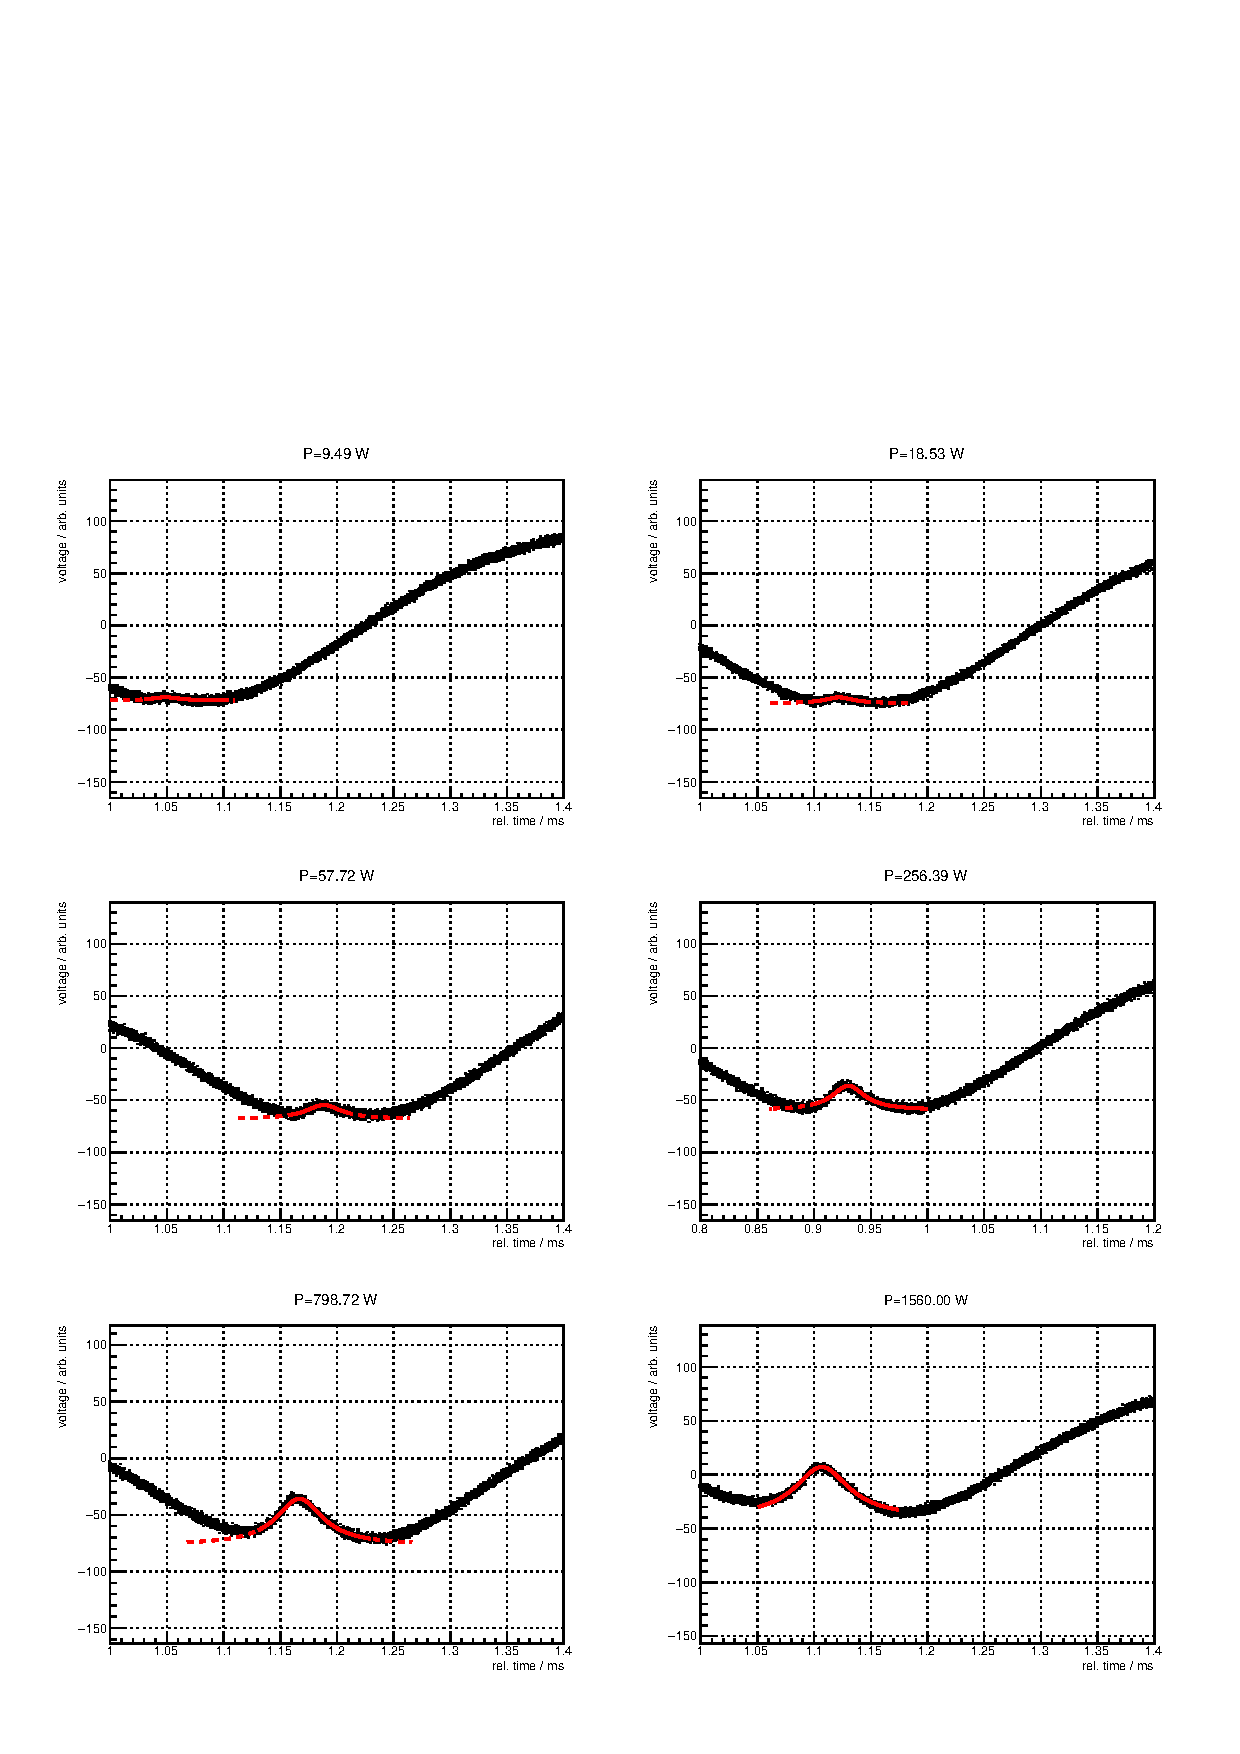
\includegraphics[width=\linewidth]{figs/measurements/widths.pdf}
	\caption{Power dependent width of the investigated peak. The \texttt{csv} file of $P=\SI{500}{\micro\W}$ was corrupted and cannot be used to fit the peak which is why we omit it here.}
	\label{fig:widthpower}
\end{figure}

\end{document}
